\chapter{Implementación digital} \chapterlabel{Informe/7-ImplementacionDigital} \label{cap:Implementacion digital}

En este capítulo se realiza el diseño de un compensador y estimador en el dominio digital para ser implementados en un microcontrolador que se conecta de manera externa a la placa de control. Para el primero se sigue la misma estrategia que se utiliza en la etapa de compensación analógica, descripta en el capítulo \ref{cap:Compensador Analogico}, pero con las consideraciones necesarias para trabajar con sistemas discretos. Para el segundo, se diseña un algoritmo encargado de obtener el valor de la distancia de separación $Y_g$ a partir de los valores obtenidos al muestrear la tensión entregada por el sensor de efecto Hall.

Por otra parte, se diseñan los circuitos de interfaz encargados de muestrear, reconstruir y adaptar los niveles de tensión de las señales que interactúan entre la placa de control y el microcontrolador.


\section{Descripción general}

 La implementación digital consiste en realizar la estimación de posición y el control de la planta por medio de un microcontrolador. Se utiliza un kit de desarrollo basado en el microcontrolador STM32F072, que contiene un conversor digital analógico (DAC) y un conversor analógico digital (ADC), ambos de 12 bits y $3.3\:V$ de referencia. 

 En la figura \ref{fig:diag-en-bloques-digital} se muestra un diagrama en bloques general de la implementación digital del sistema. Es posible observar que se ingresa al microcontrolador a través de un canal del ADC, con una tensión de referencia ($V_{y_{ref}}$) proporcional a la distancia de separación deseada, que es la misma utilizada en la implementación analógica. Además, se ingresa por medio de otro canal del ADC con la tensión de salida del sensor de efecto hall ($V_{IL_{feed}}$). Por otro lado, mediante un DAC, se ingresa al controlador de corriente $G_{IL}(s)$, que actúa sobre la planta $G_P(s)$, y modifica la distancia de separación.

% Por medio de un ADC y el sensor de efecto Hall, se muestrea una tensión proporcional a la corriente que circula por el electroimán. Se implementa un algoritmo de estimación dentro del microcontrolador que permite obtener una posición estimada $Y(z)$. Este está representado por la transferencia $H(Z)$.


\begin{figure}[H]
	\centering
	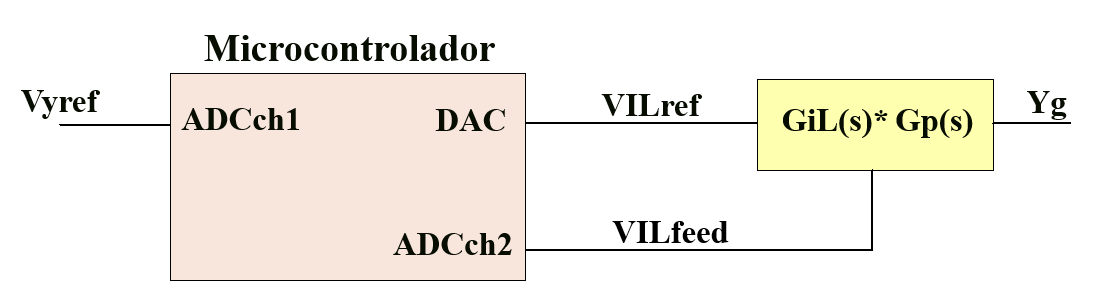
\includegraphics[scale=0.5]{Diagrama-en-bloques-digital2.png}
	\caption{Diagrama en bloques de la implementación digital.}
	\label{fig:diag-en-bloques-digital}
\end{figure}


%\colorbox{blue}{yo dejaría el de arriba que representa mejor que la entrada al sistema digital es la corriente. pero el de abajo nos sirve para el diseño del compensador también}
%
%Abstrayéndose de la matemática que se realiza dentro del microcontrolador para la estimación de posición, se puede simplificar el diagrama al que se muestra en la figura \ref{fig:diag-en-bloques-digital-simplif}, en la que:

%\begin{equation} 
%	G_T(s) = G_P(s) * G_{iL}(s).
%\end{equation}

%\begin{figure}[H]
%	\centering
%	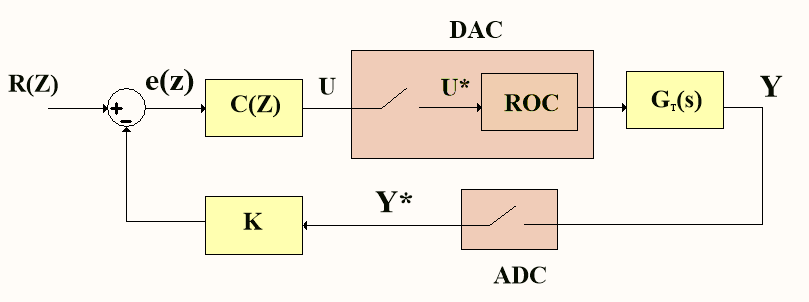
\includegraphics[scale=0.5]{Diagrama-en-bloques-digital-simplificado.png}
%	\caption{Diagrama en bloques de la etapa digital simplificado.}
%	\label{fig:diag-en-bloques-digital-simplif}
%\end{figure}
%
%\colorbox{blue}{acá arrancaría con una sección general que sea algoritmo de estimación y dentro de ella iría lo de frecuencia de muestreo, etc...}

% En la figura \ref{fig:diag-en-bloques-digital} se muestra un diagrama en bloques general de la implementación digital del sistema. Todos los bloques dentro del microcontrolador están representados por funciones transferencia en el dominio de la variable Z. \colorbox{red}{creo que sería medio complicado explicar qué es z}. Es posible observar que se ingresa al microcontrolador a través de un ADC, con una tensión de referencia ($V_{y_{ref}}$) proporcional a la distancia de separación deseada, que es la misma utilizada en la implementación analógica. Esta es multiplicada por la ganancia de entrada $G_{in}$ y luego es comparada con la posición estimada $Y(z)$. El resultado $e(z)$ es la entrada del compensador digital $C(z)$. Por medio de un DAC, la salida del compensador digital ingresa al controlador de corriente $G_{IL}(s)$, que actúa sobre la planta $G_P(s)$, y modifica la distancia de separación.
%
%Por medio de un ADC y el sensor de efecto Hall, se muestrea una tensión proporcional a la corriente que circula por el electroimán. Se implementa un algoritmo de estimación dentro del microcontrolador que permite obtener una posición estimada $Y(z)$. Este está representado por la transferencia $H(Z)$.
%
%\colorbox{blue}{yo dejaría el de arriba que representa mejor que la entrada al sistema digital es la corriente. pero el de abajo nos sirve para el diseño del compensador también}
% Abstrayéndose de la matemática que se realiza dentro del microcontrolador para la estimación de posición, se puede simplificar el diagrama al que se muestra en la figura \ref{fig:diag-en-bloques-digital-simplif}, en la que:
%
%\begin{equation} 
%	G_T(s) = G_P(s) * G_{iL}(s).
%\end{equation}
%
%\begin{figure}[H]
%	\centering
%	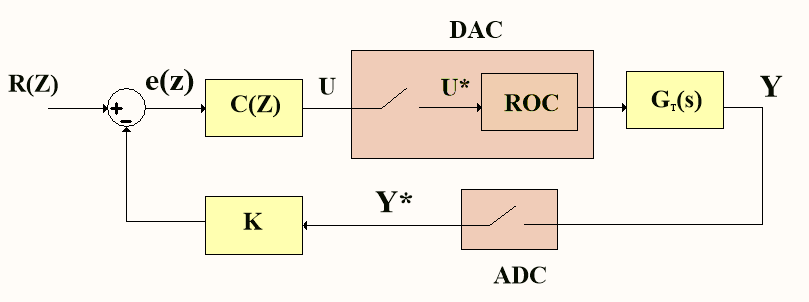
\includegraphics[scale=0.5]{Diagrama-en-bloques-digital-simplificado.png}
%	\caption{Diagrama en bloques de la etapa digital simplificado.}
%	\label{fig:diag-en-bloques-digital-simplif}
%\end{figure}
%
%\colorbox{blue}{acá arrancaría con una sección general que sea algoritmo de estimación y dentro de ella iría lo de frecuencia de muestreo, etc...}


\section{Consideraciones para el dominio discreto}

Como se menciono previamente para la implementación digital se van a tomar muestras de la señales de la planta y se las van a utilizar para implementar un algoritmo de compensación dentro del microcontrolador. 

Como se ve en la figura \ref{fig:diag-en-bloques-digital} se tiene un compensador en el dominio discreto, pero se desea controlar una planta que es continua. Para convertir senales analógicas a discretas y viceversa para poder ser utilizadas en el algoritmo de control se utilizan conversores analógico digitales ($ADC$) y conversores digital analógicos ($DAC$) 

Para hacer esta conversion los dispositivos mencionados mantienen el valor entre muestra y muestra, actualizando el valor de la senial en cada intervalo de tiempo discreto. Este efecto se lo conoce como retenedor de orden cero ($ROC$) y se lo puede modelar con la siguiente ecuación:

\begin{equation*}
	ROC(s)=\frac{1-e^{-s*T_s}}{s}
\end{equation*}

Luego de realizar la conversión, teniendo en cuenta el efecto del $ROC$, como se esta trabajando en con un modelo discreto se debe aplicar la transformada $Z$ de las seniales continuas. Por lo tanto ahora las seniales muestreadas en el microcontorlador para una entrada entrada($R(t)$) en el plano S son:

\begin{equation*}
	R(z)= Z[ROC(s)*R(s)]
\end{equation*}

Trabajando en el plano Z se puede diseniar un compensación digital ($G_c(z)$) a partir de las diferencia ($E(z)$) entre las seniales de entrada al microcontrolador  correspondientes a la señal de referencia ($V_{iLref}$) y la de realimentación de la corriente ($V_{iLfeed}$).  

\begin{equation*}
	G_c(z)=\frac{U(z)}{E(z)}
\end{equation*}

Para poder diseñar esta compensación digital, se pueden aplicar herramientas que permiten aplicar técnicas de diseño para sistemas continuos y obtener su equivalente en el plano transformado Z para ser implementado en el microcontrolador.

Esta herramienta es la transformada bilineal. Por medio de esta es posible diseñar un compensador con técnicas de compensación analógico y luego, con su transformada inversa, obtener el compensador en el dominio discreto. Esta transformada consiste en aplicar la siguiente ecuación: 

\begin{equation*}
	z=\frac{1+sT_s}{1-sT_s}
\end{equation*}


\subsection{Transferencias de la planta y del controlador de corriente}

Para el análisis del compensador digital se parte de las transferencias de la planta $G_P(s)$ y del controlador de corriente $G_{iL}(s)\ $ en dominio analógico para una masa de $30 \:kg$.

\begin{equation} 
	\begin{aligned}
		G_T(s)[M=30kg]&=G_P(s)*G_{iL}(s)&=\frac{-87.7}{\ (s-70)\ (s+70)\ (s+12.17)}\\
	\end{aligned}
\end{equation}

Para incluir el efecto del ROC a esta transferencia se aplica la transformada z por el método de invarianza al impulso. Aplicando propiedades se obtiene que 

\begin{equation*}
	\frac{Y(z)}{R(z)}=Z[\frac{(1-e^{-s*T_s})}{s}*G_T(s)]=(1-z^{-1})*Z[\frac{G_T(s)}{s}])
\end{equation*}

Para obtener esta transformada es necesario conocer la frecuencia de muestreo $F_s$. A continuación se hara un análisis de cual sera el algoritmo de control y se escoge una $F_s$ para luego obtener la transferencia del controlador $G_c(z)$.
\colorbox{red}{Hacer referencia a cuando elegimos esta frecuencia}

\colorbox{red}{Escribir la expresión de la transformada z invarianza al impulso}

Por lo tanto se decide usar la misma estrategia utilizada en el compensador analógico, planteando dos lazos de realimentación: uno interno y otro externo. El primero con el objetivo de estabilizar la planta y el segundo para mejorar la respuesta temporal del sistema.  

\colorbox{red}{ponemos diagrama general de la compensación?}en este diagrama ponemos el H y aclaramos que es =1 como se disñó en al secciòn...

\section{Diseño de algoritmo de estimación}

En esta sección se diseña el algoritmo que realiza la estimación de distancia de entrehierro $Y_g$ a partir de las muestras tomadas por el ADC de la tensión de salida del sensor de efecto Hall.

La señal que entra al ADC es la salida del sensor de efecto Hall $V_{IL_{feed}}$, que está dada por:

\begin{equation*}
	V_{IL_{feed}}=K_h*I_L+0.1\:V
\end{equation*}

Donde $K_h$ es la ganancia del sensor de efecto Hall. Como la señal $V_{IL_{feed}}$ tiene un punto de operación de $0.1\:V$, se decide realizar el análisis adoptando una nueva señal $V_h$ tal que:

\begin{equation*}
	V_h=V_{IL_{feed}}-0.1\:V=K_h*I_L
\end{equation*}

\colorbox{blue}{pongo acá Vh por que la usamos mas abajo en la estimación}

La conversión entre la señal $V_{IL_{feed}}$ y $V_h$ será realizada por una etapa circuital de acondicionamiento de la señal de entrada al ADC.

La estimación de distancia de entrehierro se obtendrá al medir la pendiente de la señal $V_h$. Dentro del microcontrolador se implementa un algoritmo para procesar las muestras y calcular la distancia estimada. 

\subsection{Determinación de la frecuencia de muestreo}

El ADC toma muestras de la señal en su entrada de manera periódica. Es importante realizar un análisis de cuál es la frecuencia con la que debe tomarlas, de manera de obtener una señal adecuada para realizar la estimación.

Como se vio en el capitulo \ref{cap:ControladorCorriente}, la forma de onda de la salida del sensor de efecto Hall es triangular y presenta una frecuencia de conmutación ($F_{planta}$) que varía en función de la distancia de entrehierro. Se puede calcular como:

\begin{equation} \label{eq_frecuencia-de-muestreo}
	F_{planta}(Y_g)=\frac{V_{cc}}{2 * L(Y_g) * \Delta I_L}
\end{equation}


Al aplicar en la ecuación \ref{eq_frecuencia-de-muestreo} los valores de inductancia ($L\:[mHy]$) obtenidos en las mediciones realizadas sobre el electroimán (ver tabla \ref{tab_mediciones_inductancia}), se calcula la frecuencia de conmutación  $(F_{planta}\:[Hz])$. Los resultados se muestran en la tabla \ref{frecuencias-calculadas}.



\begin{table}[H]
	\begin{center}
		\begin{tabular}{| c | c | c |}
			\hline
			$Y_g\:[mm]$ & $L\:[mHy]$ & $F_{planta}\:[Hz]$\\ \hline
			2 & 22.64 & 1060\\ \hline
			3 & 18.8 & 1276\\ \hline
			4 & 16.44 & 1459\\ \hline
			5 & 14.9 & 1632\\ \hline
		\end{tabular}
		\caption{Valores de frecuencia calculados a partir de las mediciones de inductancia realizadas.}
		\label{frecuencias-calculadas}
	\end{center}
\end{table}


 Para la estimación de distancia de entrehierro es necesario medir la pendiente de la onda triangular sin alterar demasiado su forma. Debido a que la conversión realizada por el ADC recorta el contenido de frecuencia de la señal a partir de la mitad de frecuencia de muestreo, se debe elegir esta última de manera que se conserve la información de la pendiente.  Por lo tanto, para reconstruirla correctamente se decide que la frecuencia de muestreo del ADC sea al menos el doble de la frecuencia de la 5° armónica para el caso de distancia de entrehierro en que $F_{planta}$ es la mayor. Para tener cierto margen, se adopta que la frecuencia de muestreo sea 2.5 veces superior. Es decir:

\begin{equation} 
	F_{ADC} \geq 2.5 * 5 * F_{planta_{max}} \Rightarrow  F_{ADC} \geq 2.5 * 5 * 1632\:Hz \Rightarrow F_{ADC} \geq 20400\:Hz
\end{equation}


 De esta forma, se adopta una frecuencia de muestreo para el ADC de  $25\:kHz$. Con este valor es posible obtener 15 muestras en un período de la triangular para el caso de $F_{planta}$ máxima. Como la señal crece o decrece durante medio ciclo, se pueden tomar 7 muestras para identificar la pendiente. En el caso de que la señal presente la $F_{planta}$ mínima, se pueden tomar 23 muestras en un ciclo. Esto se traduce en 11 muestras para la pendiente de subida o bajada. 


\subsection{Adquisición y procesamiento de las muestras}

En esta sección se desarrolla el algoritmo ideado para estimar la distancia de entrehierro. Este se puede observar en el diagrama de flujo \ref{fig:procesamiento-muestras-adquiridas}. Se realiza un análisis para el caso de máxima frecuencia de conmutación, en el que solo se pueden tomar 7 muestras durante el tiempo de crecimiento o decrecimiento.


\begin{figure}[H]
	\centering
	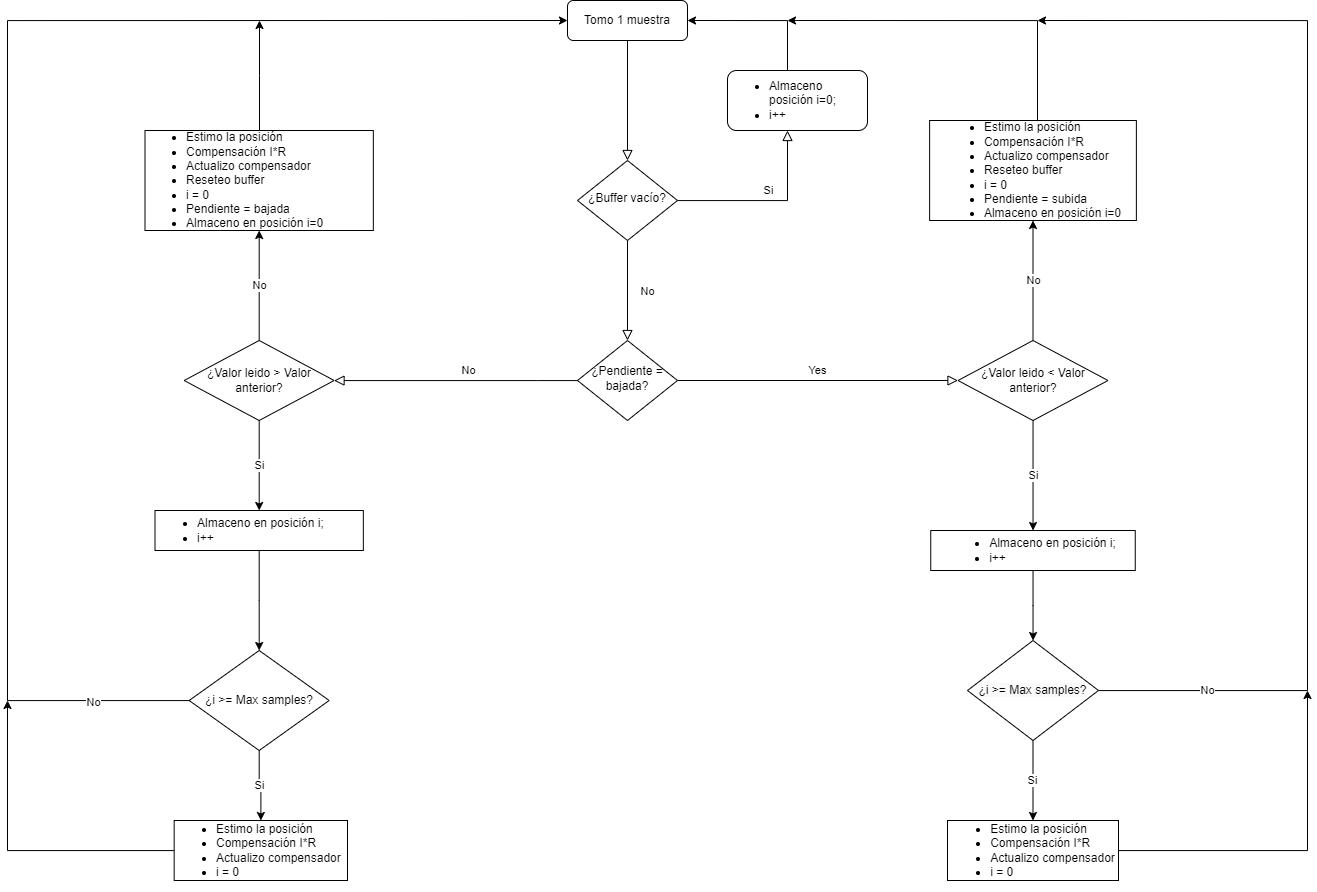
\includegraphics[scale=0.55]{Procesamiento-muestras-adquiridas.png}
	\caption{ Diagrama de flujo del procesamiento de las muestras adquiridas.}
	\label{fig:procesamiento-muestras-adquiridas}
\end{figure}


Como se observa en el diagrama de flujo de la figura \ref{fig:procesamiento-muestras-adquiridas}, cada muestra de tensión tomada de la señal $V_h$ se almacena en un \colorbox{red}{vector en memoria podría ser en español?}buffer de 7 posiciones. Para poder discernir entre pendientes de bajada y de subida, se verifica en cada muestra si el valor leído es mayor o menor al almacenado en la posición anterior. En caso de que sea mayor al anterior, significa que se está muestreando la pendiente positiva de la onda triangular. La distinción entre pendientes positivas y negativas es importante puesto que permite aplicar la compensación de la resistencia interna al igual que se realiza en el estimador analógico. 

Cada vez que el buffer se completa, se realiza el cálculo de la derivada con el valor máximo y mínimo almacenado. Con este resultado, se hace la estimación de la posición y se actualiza la entrada al compensador digital.

En caso de haber completado las 7 posiciones del buffer y la pendiente persiste con el mismo signo, el buffer comienza a llenarse nuevamente desde la posición inicial, sobrescribiendo los valores mas antiguos. Por lo tanto, pueden ocurrir dos situaciones. La primera es que se detecte un cambio de pendiente antes de completar nuevamente el buffer, con lo cual se calcula la derivada con los valores extremos almacenados teniendo en cuenta el tiempo transcurrido ($K$ períodos de muestreo), y se actualiza la entrada al compensador. La segunda, es que se vuelva a completar el buffer, en cuyo caso también se hace la actualización. La diferencia entre estas dos situaciones es el tiempo transcurrido hasta que se obtiene nueva estimación. En este último, se hace cada 7 períodos de muestreo mientras que en el primero se realiza en “N” períodos luego de la última actualización, siendo “N” la cantidad de muestras que se almacenaron en el buffer incompleto.

Luego de detectar un cambio de pendiente, el
proceso vuelve a iniciar con el buffer vacío.

Al utilizar este método de estimación, puede ocurrir que se obtenga una nueva estimación en 7 periodos de muestreo del ADC, o incluso en menos. Por lo tanto se tiene un estimador de distancia de entrehierro con frecuencia de actualización variable. Esto será importante luego al momento de diseñar el compensador digital. Para hacerlo, se debe considerar el caso en que la frecuencia de actualización es la menor. Por lo tanto el compensador digital se debe diseñar con una frecuencia de muestreo de $F_S=25/7 \:kHz = 3.5\:kHz$.

\subsection{Estimación digital de la posición}

En el capitulo \ref{cap:Estimador Analogico} se analizó la relación entre la distancia del entrehierro con la pendiente de la corriente en el electroimán. Se llegó a la expresión \ref{eq_Yg_despejada}, que se repite a continuación:

\begin{equation} \label{eq_yg_vs_derivada}
	Y_g = 5.136*10^{-6}*|\frac{di_L}{dt}|- 3.472*10^{-3} [m]
\end{equation}

A partir de la expresión \ref{eq_yg_vs_derivada} se puede obtener la distancia de entrehierro midiendo la pendiente de la corriente. Sin embargo, esta expresión fue calculada suponiendo que no se generaba una caída de tensión en la resistencia interna del electroimán ($R_L$), obteniendo una pendiente teórica. Esta caída provoca que la tensión efectiva aplicada sobre la inductancia sea distinta para el semiciclo de subida que para el de bajada. De esta forma, la onda triangular presenta diferentes pendientes (en valor absoluto) para cada caso. Esta se representa como $(\frac{di_L}{dt})_{Real}$ y es la que se mide al utilizar el ADC. La relación entre esta y la teórica se da por:

\begin{equation} \label{eq_derivada_real}
	(\frac{di_L}{dt})_{Real}=(\frac{di_L}{dt})_{Teorica}-\frac{R_L*I_L}{L(Y_g)}
\end{equation}

Por lo tanto al despejar la derivada teórica de la expresión \ref{eq_derivada_real} se obtiene:

\begin{equation} \label{eq_derivada_teorica}
	(\frac{di_L}{dt})_{Teorica}=(\frac{di_L}{dt})_{Real}+\frac{R_L*I_L}{L(Y_g)}
\end{equation}


Para calcular la derivada real de la pendiente dentro del microcontrolador se aproxima como la resta entre la muestra de corriente en un instante ($I_L[n]$) menos la muestra mas vieja en el buffer ($I_L[n-K]$) sobre el intervalo de tiempo transcurrido entre ellas ($K*T_S=\frac{K}{F_S}$). Al considerar este cálculo de la derivada y utilizar \ref{eq_derivada_teorica} en \ref{eq_yg_vs_derivada}, se obtiene:

\begin{equation} \label{eq_yg_vs_IL}
	Y_g[n] = 5.136*10^{-6}* |\frac{I_L[n]-I_L[n-K]}{K*T_S}+\frac{R_L*I_L[n]}{L(Y_g)[n-1]}| - 3.472*10^{-3} [m]
\end{equation}

$V_h$ es la tensión proporcional a la corriente que circula por el electroimán multiplicada por la ganancia $K_h=53.3\:mV/A$. Esta señal se puede separar en dos componentes: $\hat{V_h}$  correspondiente a la componente alterna de tensión y $\bar{V_h}$ a la continua:


\begin{equation} 
	V_h[n] = \bar{V_h}[n] + \hat{V_h}[n] = K_h * (\bar{I_L}[n] + \hat{I_L}[n])
\end{equation}

 Para la estimación de la posición se utiliza el término de alterna mientras que para compensar el error introducido por la resistencia interna del electroimán se utiliza el de continua. Por lo tanto reemplazando $I_L=\frac{V_h}{K_h}$ en la ecuación \ref{eq_yg_vs_IL}, se obtiene:

\begin{equation}
	\resizebox{.8\hsize}{!}
	{
	$Y_g[n] = 5.136*10^{-6}*|\frac{\hat{V_h}[n]-\hat{V_h}[n-K]}{K*K_h*T_S} + \frac{R_L*\bar{V_h}[n]}{K_h*L(Y_g)[n-1]}|-3.472*10^{-3}[m]$
	}
\end{equation}

El término $\bar{V_h}[n]$ se obtiene de sensar el valor medio de la tensión $V_h$ mediante un canal del ADC.

Por otro lado, el valor de $L(Y_g)[n-1]$ se obtiene al aplicar el valor estimado de posición anterior en la ecuación \ref{eq_inductancia}. El cálculo de esta expresión se obtuvo a partir de la linealización de la inductancia en función de las mediciones realizadas sobre el electroimán.


\begin{equation} \label{eq_inductancia}
	L(Y_g)[n] = -2.56*Y_g[n]+0.0271\:Hy
\end{equation}

 Por lo tanto, la ecuación correspondiente en el tiempo discreto resulta:

\begin{equation}
	\resizebox{.8\hsize}{!}
	{
	$Y_g[n] = 5.136*10^{-6}*|\frac{\hat{V_h}[n]-\hat{V_h}[n-K]}{K*K_h*T_S} + \frac{R_L*\bar{V_h}[n]}{K_h*(2.56*Y_g[n-1]+0.0271)}|-3.472*10^{-3}\:[m]$
	}
\end{equation}

\begin{equation}
	\resizebox{.8\hsize}{!}
	{
	$
	Y_g[n] = 96.3*10^{-6}*|\frac{\hat{V_h}[n]-\hat{V_h}[n-K]}{K*T_S} + \frac{R_L*\bar{V_h}[n]}{(2.56*Y_g[n-1]+0.0271)}|-3.472*10^{-3}\:[m]
	$
	}
\end{equation}


El número de muestras está representado por ``n''. Es decir, $V_h[n]$ se refiere a la muestra más reciente en el buffer y $V_h[n-K]$ a la más vieja.

Es importante notar que los coeficientes del estimador deben calcularse justo antes de realizar una nueva estimación,  en función de la cantidad de muestras que se utilizan para el cálculo de la pendiente. Si bien el estimador presenta una frecuencia de actualización variable, los coeficientes del compensador digital no se ven modificados ya que se calculan teniendo en cuenta la frecuencia de actualización más lenta.

Por otro lado, el bloque $H_D$ mostrado en la figura \ref{fig:diag-en-bloques-digital-simplif} resulta en una transferencia unitaria.
 \colorbox{red}{si sacamos la figura hay que ver de modificar esto o sacarlo}

\subsection{Resolución en posición}

En esta sección se analiza cuál es la resolución en posición que se puede obtener con el algoritmo de estimación diseñado.

Una variación de posición ($\Delta Y_g$) produce un cambio de inductancia ($\Delta L(Y_g)$) que se traduce en un cambio de frecuencia ($\Delta F_{planta}$). Para poder detectar el mínimo cambio de posición en un período de muestreo se debe tener una resolución tal que permita discernir ese cambio de frecuencia.


A partir de la expresión linealizada de la inductancia \ref{eq_induct_practica} y la ecuación \ref{eq_frecuencia-de-muestreo} es posible obtener el valor de frecuencia para una separación de $Y_g=2.1\:mm$. Esta resulta en $F_{planta}[2.1\:mm] = 1104.8\:Hz$. De esta forma, al conocer el valor de frecuencia para $2\:mm$, el cual es de $F_{planta}[2\:mm] = 1060\:Hz$, es posible obtener la variación de frecuencia para un ($\Delta Y_g$) mínimo de  $0.1\:mm$. Este valor puede obtenerse como:

\begin{equation} 
	\Delta F_{planta} = F_{planta}[2.1\:mm] - F_{planta}[2\:mm] = 44.8\:Hz
\end{equation}

 Las pendientes para el peor caso se da con la menor variación de tensión entre muestras. Es decir, para el caso de en que $F_{planta}$ es la mínima. En la ecuación \ref{eq_pendiente} se muestra el cálculo de la pendiente de la onda triangular en función de la frecuencia de conmutación.

\begin{equation} \label{eq_pendiente}
	P(F_{planta}) = \frac{\Delta V}{T_{planta}/2} = 2*K_h*\Delta i_L*F_{planta} = 2 * 0.0533 * 0.5 * F_{planta}
\end{equation}

 A partir de la ecuación \ref{eq_pendiente} es posible obtener el valor de la pendiente para la mínima frecuencia de conmutación y la de su incremento correspondiente a una variación en la posición de $0.1\:mm$. Esta situación se representa en la figura \ref{fig:variacion-de-pendiente}.

\begin{equation} 
	\begin{aligned}
		&P(F_{planta_{min}}) = 56.49\:[V/s] \\
		&P(F_{planta_{min}} + \Delta F_{planta}) = 58.89\:[V/s] \\
	\end{aligned}
\end{equation}

\begin{figure}[H]
	\centering
	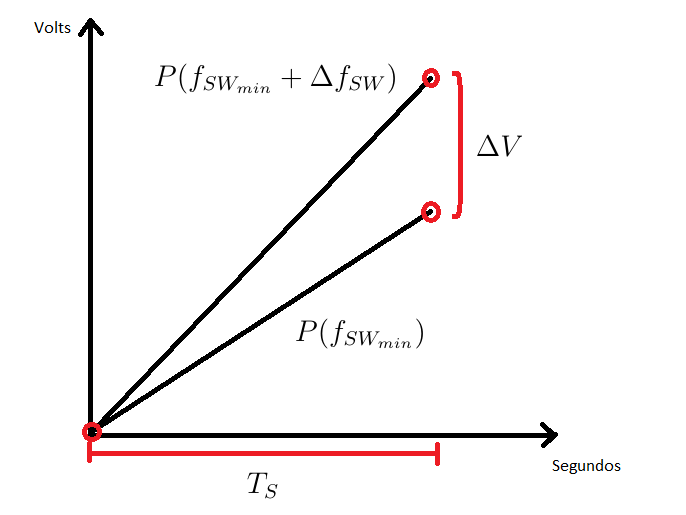
\includegraphics[scale=0.5]{Variacion-de-pendientes.png}
	\caption{Variación de pendiente ante mínimo cambio de posición.}
	\label{fig:variacion-de-pendiente}
\end{figure}

\colorbox{red}{en el texto antes deciamos Fplanta y fsw como que eran lo mismo. cambié todas por Fplanta pero en la imagen quedó com fsw... que hacemos?}

 Por lo tanto, para poder diferenciar las pendientes, la resolución del ADC debe ser menor o igual a $\Delta V$.

\begin{equation} 
	\begin{aligned}
		V1 &= P(F_{planta_{min}} + \Delta F_{planta})* T_{ADC} \\
		V2 &= P(F_{planta_{min}})* T_{ADC} \\		 
	\end{aligned}
\end{equation}

 Al considerar $F_{ADC} = 25\:kHz$:

\begin{equation} 
	\Delta V_{ADC} = T_S * [P(F_{planta_{min}} + \Delta F_{planta}) - P(F_{planta_{min}})] = 96\:\mu V
\end{equation}



 Este resultado indica que se necesita una resolución en el ADC de $96\:\mu V$. Este valor depende de la cantidad de bits (N) que utiliza el ADC y de su tensión de referencia ($V_{ref}$), de manera que:
 
 \begin{equation*}
 	\Delta V_{ADC}=\frac{V_{ref}}{2^N}
 \end{equation*}

Al usar un ADC de 12 bits, se necesitaría una tensión de referencia $V_{ref} = 0.39\:V$ para lograr la resolución de $96\:\mu V$. Sin embargo, este valor resulta demasiado bajo y no sirve si se quiere medir la tensión de salida del sensor de efecto Hall de manera directa. Por lo tanto, se decide diseñar un circuito que permita realizar la estimación manteniendo la tensión de referencia en $3.3\:V$ y teniendo una resolución $\Delta V_{ADC}=0.8\:mV$.

\subsection{Adaptación de señal de entrada al ADC}

En esta sección se analiza una estrategia para poder medir la señal $V_h$ con la precisión deseada.

La corriente que circula por el electroimán presenta una componente de continua y otra de alterna. La primera excursiona entre $0\:A$ y $30\:A$ mientras que la segunda varía entre $\pm 250\:mA$ en torno al valor medio, con forma de onda triangular. Esto significa que la señal $V_h$ está compuesta por un valor medio que varía entre $0\:V$ y $1.6\:V$, y un valor de alterna de $26.7\:mV_{pp}$.

Se propone realizar una adquisición separada de ambas componentes de la tensión $V_h$. De esta manera se puede ingresar a un canal del ADC con $\bar{V_h}$ y en otro canal ingresar con $\hat{V_h}$. Esto permite amplificar la señal $\hat{V_h}$ para lograr la resolución deseada. Además se agrega un punto de operación de $2.5\:V$ a esta señal amplificada.

Debido a que el ADC permite una excursión entre $0\:V$ y $3.3\:V$, la máxima ganancia posible es de 60 veces para la componente de alterna.

\begin{equation*}
	3,3 \:V = \frac{26.7\:mV_{pp}}{2}*G_{max}+2,5\:V
\end{equation*}


Por otro lado, para medir con la resolución en posición deseada de $0.1\:mm$ se la debe amplificar 9 veces como mínimo.

\begin{equation*}
	0,8\:mV_{pp} = 96\:\mu V * 9
\end{equation*}

Por lo tanto, se adopta una ganancia de 50, y se obtiene una excursión máxima de $3.17\:V$ (es decir, $0.67\:V$ sobre el punto de operación).

Para realizar la separación de las componentes de la señal $V_h$ se utiliza un circuito con las siguientes características:

\begin{itemize}
	\item Ganancia: 50
	\item \textsl{set-point} de $2.5\:V$
	\item Frecuencia de corte inferior: $100\:Hz$
	\item Frecuencia de corte superior: $12,5\:kHz$
\end{itemize}

La frecuencia de  corte superior de $12,5\:kHz$ corresponde a la de un filtro antialiasing. El uso de estos filtros antes de la discretización de los datos es necesario ya que al hacerlo aparece una réplica espectral de la señal muestreada desplazada a la frecuencia de muestreo y a sus n-múltiplos. Esta réplica puede mezclarse con la señal deseada. 

Al considerar la ganancia elegida,  la pendiente de la onda triangular resulta:

\begin{equation} 
	P(F_{planta}) = 50 * [0.0533 * 0.5 * (F_{planta}*2)]\:[\frac{V}{s}]
\end{equation}

 Al reemplazar para el incremento de frecuencia se obtiene: 

\begin{equation} 
	\begin{aligned}
		&P(F_{planta_{min}}) = 2824.9 \: [\frac{V}{s}]\\
		&P(F_{planta_{min}} + \Delta F_{planta}) = 2944.29 \: [\frac{V}{s}]\\		 
	\end{aligned}
\end{equation}

 Por lo tanto, resulta:


\begin{equation} 
	\resizebox{.8\hsize}{!}
	{
	$\Delta V_{ADC} = T_S * [P(F_{planta_{min}} + \Delta F_{planta}) - P(F_{planta_{min}})] = 0.1177\:V - 0.1129\:V = 4.7\:mV$
	}
\end{equation}


 De esta manera, como la resolución del ADC es de $0.8\:mV$, resulta suficiente para identificar el mínimo cambio de pendiente.


\section{Circuitos de acondicionamiento de señales para el ADC}

\subsection{Referencia de posición}

 Para indicar al microcontrolador la distancia de separación deseada se utiliza una señal continua como referencia que se ajusta desde un potenciómetro ubicado en la placa de control  e ingresa al circuito mostrado en la figura \ref{fig:circuito-ref-posicion}. Esta señal de referencia es también utilizada por el compensador analógico. Debido a que entrega una tensión entre $3.96\:V$ y $4.69\:V$, se implementa un circuito de acondicionamiento.

 A la señal de entrada se le resta el punto de operación de $2.5\:V$, para lograr señales que van desde $1.42\:V$ a $2.2\:V$. Luego, dentro del microcontrolador, se debe asignar cada valor leído por el ADC a una distancia de separación deseada utilizando la ganancia del estimador analógico según la expresión \ref{eq_y-ref-dig}. Además se implementa un filtro \textsl{anti-aliasing} con frecuencia de corte en $9.9\:kHz$. \colorbox{red}{Pq elegimos esta frecuencia? Habría que justificarlos creo}

\begin{equation} \label{eq_y-ref-dig}
	Y_{ref}\ =\frac{Vpo{s_{ref}}_{ADC}\ +\ 2.5\:V}{259.6}\:[m]
\end{equation}

\begin{figure}[H]
	\centering
	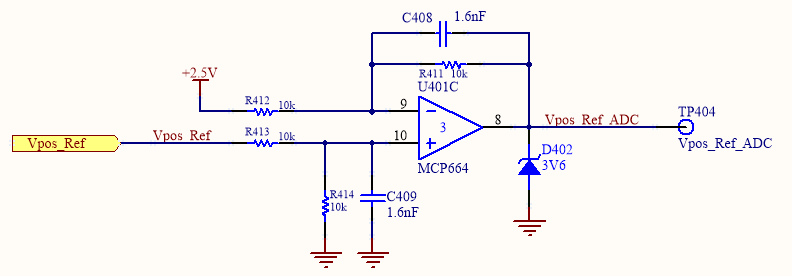
\includegraphics[scale=0.5]{Circuito-ref-posicion.png}
	\caption{Circuito acondicionador para referencia de posición.}

\end{figure}

\begin{figure}[H]
	\centering
	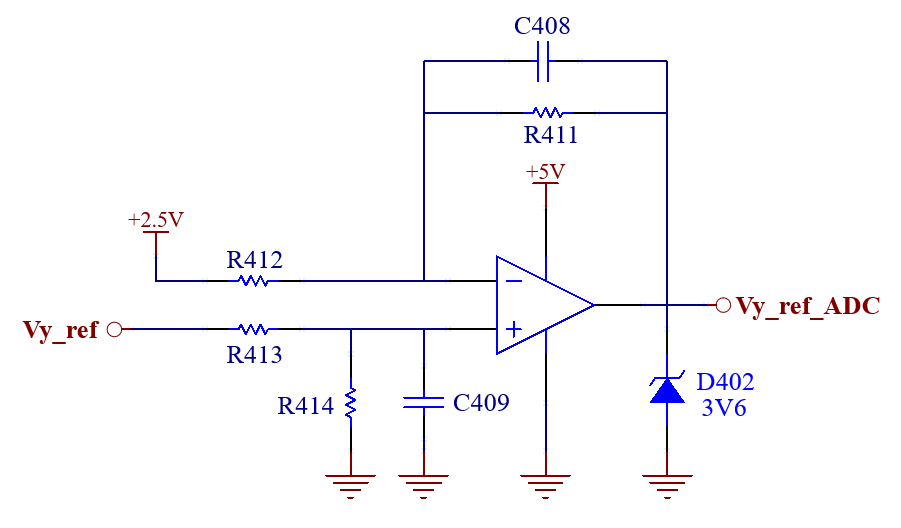
\includegraphics[scale=0.5]{Circuito-ref-posicion_dig.png}
	\caption{Circuito acondicionador para referencia de posición.}
	\label{fig:circuito-ref-posicion}
\end{figure}


Se considera que:

\begin{equation*} 
	Z=\frac{1}{sc_{408}}//R_{411}=\frac{1}{sc_{409}}//R_{414}
\end{equation*}

La salida del circuito queda como:

\begin{equation*} 
	V_{pos\_Ref\_ADC}=\frac{Z}{Z+R_{413}}(1+\frac{Z}{R_{412}})V_{pos\_Ref}-\frac{Z}{R_{412}}*2.5\:V
\end{equation*}

Si se considera que $R_{412}=R_{413}$ resulta:

%y que $2.5\:V$ es una señal continua se obtiene:
\begin{equation*} 
	V_{pos\_Ref\_ADC}=\frac{Z}{R_{412}}V_{pos\_Ref}-\frac{Z}{R_{412}}*2.5\:V
\end{equation*}


Si se considera que $R_{411}=R_{412}$ y que $2.5\:V$ es una señal continua se obtiene:

\begin{equation*} 
	V_{pos\_Ref\_ADC}=\frac{1}{1+sC_{408}R_{411}}V_{pos\_Ref}-2.5\:V
\end{equation*}

\begin{equation*} 
	\frac{V_{pos\_Ref\_ADC}}{V_{pos\_Ref}}=\frac{R_{411}*(R_{413}+R_{414})}{R_{413}*(R_{411}+R_{412})}*\frac{sC_{408}(R_{411}//R_{412})+1}{(sC_B(R_{413}//R_{414})+1)*(sC_{408}R_{411}+1)}
\end{equation*}

Por lo tanto, para obtener una frecuencia de corte para el filtro \textsl{anti-aliasing} de $9.9\:kHz$ se elige $R_{411}=50\:k\Omega$ y resulta $C_{408}=1.6\:nF$. De esta forma, se obtiene que $R_{412}=R_{413}=R_{414}=50\:k\Omega$ y que $C_{409}=1.6\:nF$.


\subsection{Componente  alterna de corriente del electroimán}

 Para obtener solamente la componente alterna de la corriente, se implementa un circuito con característica pasa-banda que se muestra en la figura \ref{fig:componente-corriente-alterna}. La frecuencia de corte inferior  es de $100\:Hz$, con el objetivo de eliminar el valor medio de señal. Por otro lado, la superior es de $12\:kHz$, que actúa como filtro \textsl{anti-aliasing}. Luego, la salida es amplificada con una ganancia de 50 veces (para mejorar la medición de la pendiente por el ADC) y se agrega un \textsl{set-point} de $2.5\:V$.

\begin{figure}[H]
	\centering
	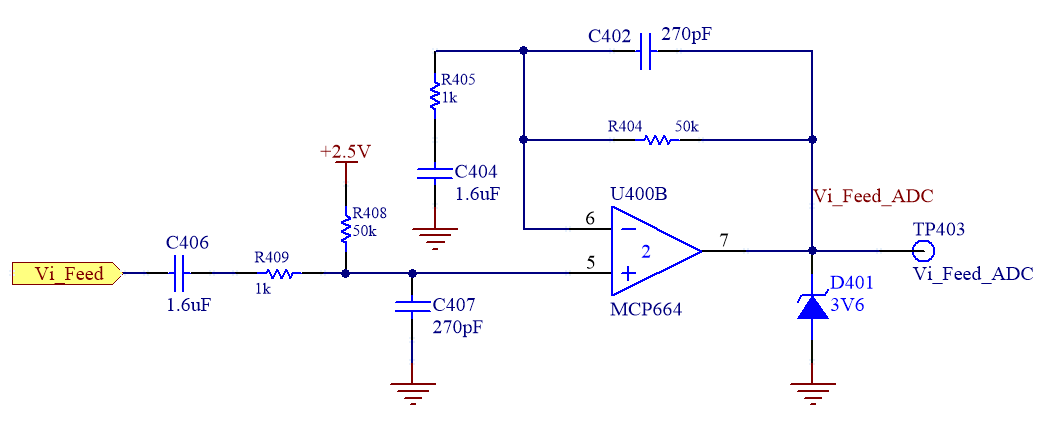
\includegraphics[scale=0.5]{Componente-corriente-alterna.png}
	\caption{ Circuito acondicionador para componente alterna de corriente del electroimán.
	}

\end{figure}

\begin{figure}[H]
	\centering
	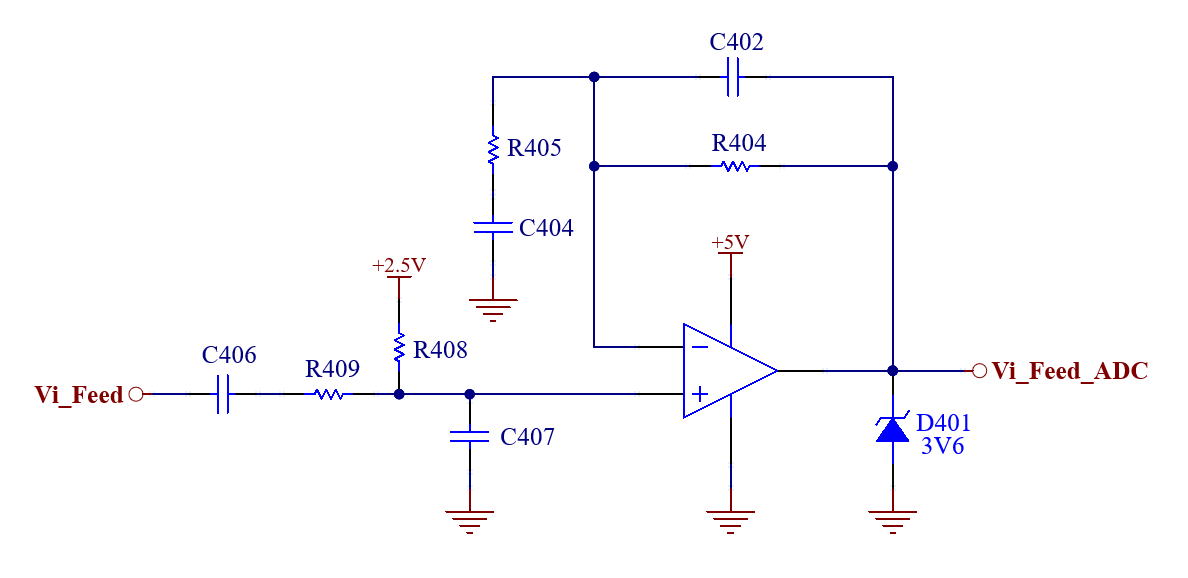
\includegraphics[scale=0.5]{Componente-corriente-alterna_dig.png}
	\caption{ Circuito acondicionador para componente alterna de corriente del electroimán.
	}
	\label{fig:componente-corriente-alterna}
\end{figure}

\subsection{Componente continua de corriente del electroimán}

 Para obtener la componente de continua se utiliza un filtro pasa-bajos con frecuencia de corte en $106\:Hz$. Se eligió esta frecuencia para que se ubique por lo menos una década por debajo de la frecuencia fundamental de la onda triangular. La implementación circuital puede observarse en la figura \ref{fig:componente-corriente-continua}

\colorbox{blue}{esta señal Vilfeed es la que tiene los 0.1V sumados? no me acuerdo si después lo cancelabamos dentro del micro}

\begin{figure}[H]
	\centering
	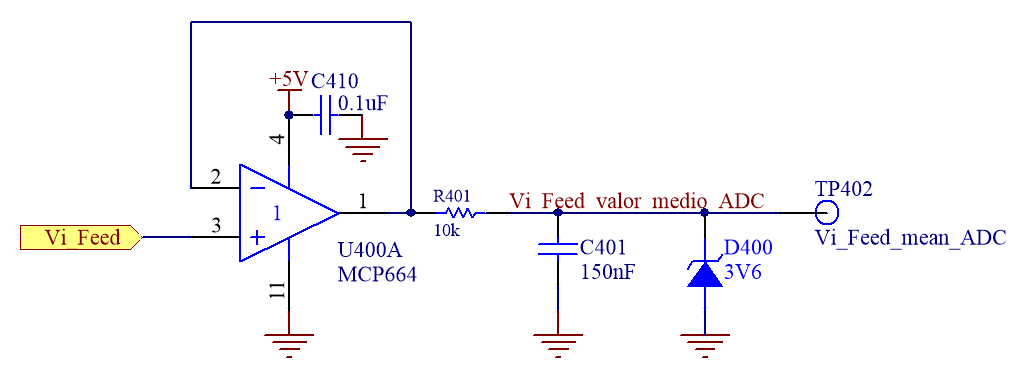
\includegraphics[scale=0.5]{Componente-corriente-continua.png}
	\caption{Circuito acondicionador para componente continua de corriente del electroimán.
	}

\end{figure}

\begin{figure}[H]
	\centering
	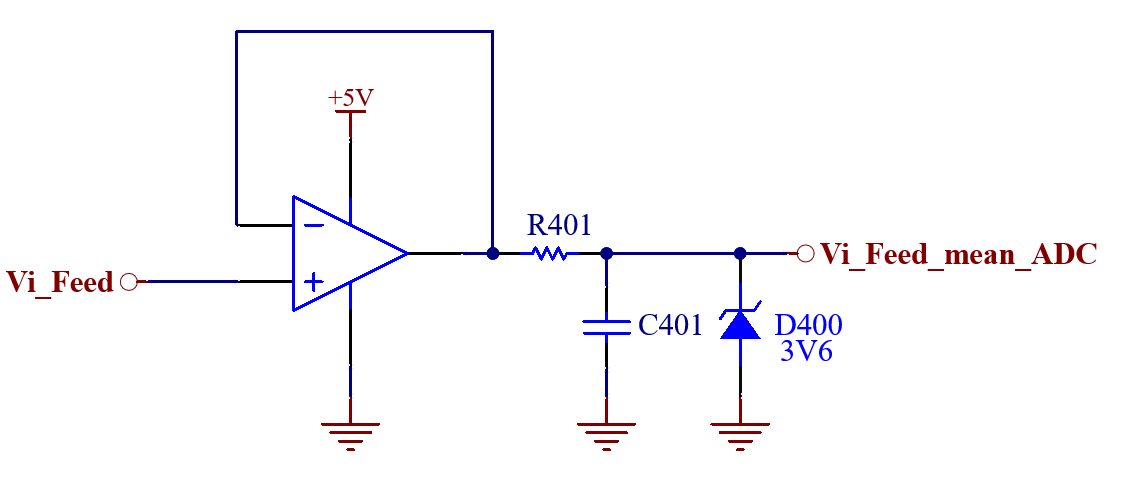
\includegraphics[scale=0.5]{Componente-corriente-continua_dig.png}
	\caption{Circuito acondicionador para componente continua de corriente del electroimán.
	}
	\label{fig:componente-corriente-continua}
\end{figure}

\begin{equation*}
	Vi\_Feed\_mean\_ADC=\frac{1}{1+sC_{401}R_{401}}*Vi\_Feed
\end{equation*}

\section{Circuitos de acondicionamiento de señales para el DAC}

 Para convertir los valores digitales de la estimación de posición y de la compensación al dominio analógico, se utiliza el DAC del microcontrolador. La tensión entregada es afectada por una circuitería de filtrado, ganancia y protección como se muestra en las figuras \ref{fig:DAC-compensador} y \ref{fig:DAC-estimador}. Debido a que el DAC se actualiza con una frecuencia mínima de $3.5\:kHz$, se utilizan filtros con frecuencia de corte en $1.75\:kHz$.

 Por otro lado, como el controlador de corriente funciona con tensiones de hasta $5\:V$ en su entrada y el compensador fue diseñado teniendo en cuenta este nivel de tensión, se agrega una ganancia por firmware de $0.66$, mapeando así los $5\:V$ a $3.3\:V$, que es la máxima tensión entregada por el DAC. Luego, para compensar esta ganancia y no afectar a la transferencia de la planta, se la afecta por un factor de $\frac{5V}{3.3V}$ por medio del circuito de acondicionamiento.

 De esta forma, se logra convertir correctamente la señal digital en analógica.


\begin{figure}[H]
	\centering
	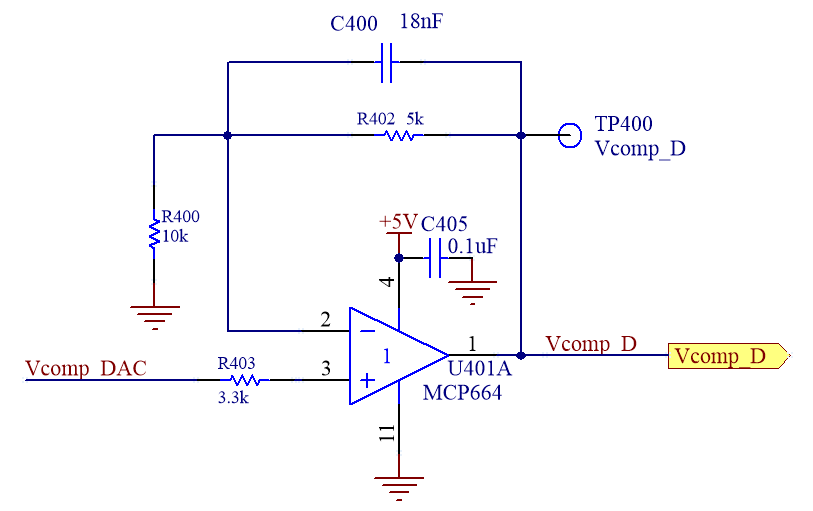
\includegraphics[scale=0.5]{DAC-compensador.png}
	\caption{Circuito acondicionador para la salida del DAC correspondiente al compensador.}
	\label{fig:DAC-compensador}
\end{figure}

\begin{figure}[H]
	\centering
	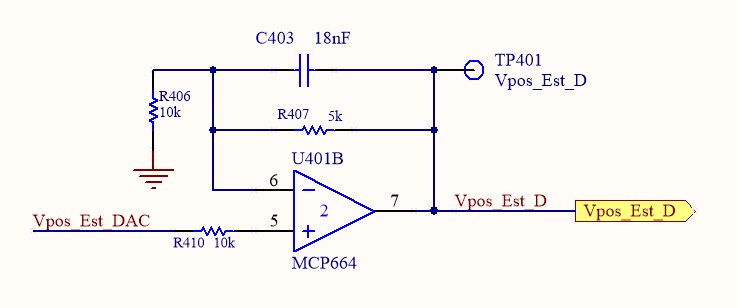
\includegraphics[scale=0.5]{DAC-estimador.png}
	\caption{Circuito acondicionador para la salida del DAC correspondiente al estimador digital.}
	\label{fig:DAC-estimador}
\end{figure}

\section{Diseño del controlador digital}


Como se menciono previamente para la implementación digital se van a tomar muestras de la señales de la planta y se las van a utilizar para desarrollar un controlador de forma digital. 

Al tomar muestras se esta discretizando una señal continua, para hacer esto, se utilizan conversores analógico digitales que mantienen el valor de esta entre muestra y muestra. Este tipo de reconstrucción de señal también se lo llama $ROC$ y se lo puede modelar con la siguiente ecuación:

\begin{equation*}
	ROC(s)=\frac{1-e^{-s*T_s}}{s}
\end{equation*}

Luego para una entrada($R(s)$) representada por un tren de pulsos con distinto valor para cada periodo de muestreo $T_s$ que ingresa a un sistema que posee una transferencia $G(s)$ se puede aplicar la transformada Z y expresar la salida como:

\begin{equation*}
	\frac{Y(z)}{R(z)}=Z[\frac{(1-e^{-s*T_s})}{s}*G(s)]=(1-z^{-1})*Z[\frac{G(s)}{s}])
\end{equation*}

Se desea implementar un algoritmo de compensación dentro del microcontrolador. Este se ejecuta cada vez que se obtiene una nueva estimación de distancia de entrehierro. Recibe en su entrada un valor correspondiente a la diferencia entre la señal de referencia y la realimentación. Este valor se denomina $e[n]$. El algoritmo de compensación realiza cálculos a partir de esta entrada y obtiene en su salida una señal $u[n]$. La relación entre $u[n]$ y $e[n]$ es una ecuación en diferencias, cuya transformada discreta (z) es la función transferencia del compensador ($G_c(z)$).

\begin{equation*}
	G_c(z)=\frac{U(z)}{E(z)}
\end{equation*}

Entonces se tiene un compensador en el dominio discreto, pero se desea controlar una planta que es continua. La forma de comunicar la salida del compensador con la entrada de la planta es mediante la utilización de un DAC. Este conlleva la ¿desventaja? de que su salida se actualiza cada intervalos de tiempo discretos. Este efecto se conoce como retenedor de orden cero (ROC), y genera un deterioro en la estabilidad del sistema. El compensador que se diseñe debe tener en cuenta este efecto.



Para poder diseñar un compensador digital para un sistema continuo, se pueden aplicar técnicas de diseño que permiten modelar la planta continua a la vez que se tiene en cuenta el efecto del ROC. De esta manera se pueden aplicar técnicas de compensación para sistemas analógicos.

\colorbox{red}{Redactar bien esta parte}
Por medio de la transformada bilinal es posible diseñar un compensador en el dominio analógico y luego, con su transformada inversa, obtener el compensador en el dominio discreto. Por lo tanto se decide usar la misma estrategia utilizada en el compensador analógico, planteando dos lazos de realimentación: uno interno y otro externo. El primero con el objetivo de estabilizar la planta y el segundo para mejorar la respuesta temporal del sistema.  

\colorbox{red}{ponemos diagrama general de la compensación?}en este diagrama ponemos el H y aclaramos que es =1 como se disñó en al secciòn...

\subsection{Transferencias de la planta y del controlador de corriente}

 Para el an\'{a}lisis del compensador digital se parte de las transferencias de la planta $G_P(s)$ y del controlador de corriente $G_{iL}(s)\ $ en dominio anal\'{o}gico para una masa de $30 \:kg$.

\begin{equation} 
	\begin{aligned}
		G_T(s)[M=30kg]&=G_P(s)*G_{iL}(s)&=\frac{-87.7}{\ (s-70)\ (s+70)\ (s+12.17)}\\
	\end{aligned}
\end{equation}

Para incluir el efecto del ROC a esta transferencia se aplica la transformada z por el método de invarianza al impulso. Con una $f_s=3.5\:kHz$, se obtiene:
 
 \colorbox{red}{Hacer referencia a cuando elegimos esta frecuencia}

\colorbox{red}{Escribir la expresión de la transformada z invarianza al impulso}

\begin{equation} 
	G_T(z)[M=30\:kg] =\frac{-3.2057*10^{-10}(z+3.729)(z+0.2677)}{(z-0.9966)(z-0.9806) (z-1.02)}
\end{equation}

Luego, se utiliza la transformada bilineal ($z=\frac{1+wT/2}{1-wT/2}$) para obtener una transferencia en el dominio analógico de la variable $w$. Considerando $T=1/f_s$:

\begin{equation}
	\resizebox{.8\hsize}{!}
	{
		$G_T(w)[M=30\:kg]\ \ =\frac{-8.0207*10^{-11}(w-1.238*10^4)(w-7143)(w+1.237*10^4)}{\ (w-70)\ (w+70)\ (w+12.17)}$
	}
\end{equation}


 Con las expresiones en $[w]$ es posible diseñar un controlador utilizando técnicas de diseño en el dominio analógico y luego transformarlo al digital nuevamente con la transformada bilineal inversa.
 
 \colorbox{red}{chequear cual es la inversa y cual la directa}

\subsection{Diseño del compensador}

Se decide usar la misma estrategia utilizada en el compensador analógico, planteando dos lazos de realimentación: uno interno y otro externo. El primero con el objetivo de estabilizar la planta y el segundo para mejorar la respuesta temporal del sistema.  

Por lo tanto, se plantea el diagrama en bloques de la figura \ref{fig:diag-en-bloques-comp_digital}

\begin{figure}[H]
	\centering
	\scalebox{0.8}{\tikzset{%
	buffer/.style={
		draw,
		shape border rotate=270,
		regular polygon,
		regular polygon sides=3,
		fill=blue!20,
		node distance=2cm,
		minimum height=4em
	}
}

\tikzstyle{block} = [draw, fill=blue!20, rectangle, 
minimum height=2.5em, minimum width=3em]

%Acá se define eñ diagrama en bloques completo
\begin{tikzpicture}[auto, node distance=1cm,>=latex']
	% We start by placing the blocks
	\node [input, name=input] {};
	\node [buffer, right=of input](F){F};
	\node [sum, right of=F, node distance=1.5cm] (suma_externa) {+};
	\node [block, right=of suma_externa] (externo) {$G_{ext}(w)$};
	\node [sum, right=of externo] (suma_interna) {+};
	\node[block, right=of suma_interna] (interno) {$G_c(w)$};
	\node [block, right=of interno] (gil) {$G_{IL}(w)$};
	\node [block, right=of gil] (planta) {$G_p(w)$};
	\node [coordinate, below=of interno] (realimentacion_interna) {$H_{estim}(w)$};
	
	\node [coordinate, below=2cm of externo] (realimentacion_externa) {$H_{estim}$};
%	
%	\node [block, right of=suma] (amplificador) {$A(s)$};
	\node [output, right of=planta, node distance=3cm] (output) {};
%	\node [block, below of=amplificador] (realimentacion) {$H(s)$};
%	
%	
%	% Once the nodes are placed, connecting them is easy. 
	\draw [draw,->] (input) -- node[pos=0.2]{$V_{y_{ref}}$} (F);
	\draw [draw,->] (F) -- node[pos=0.9]{$+$}(suma_externa);
	\draw [draw,->] (suma_externa) -- (externo);
	\draw [draw,->] (externo) -- node[pos=0.95]{$+$} (suma_interna);
	\draw [draw,->] (suma_interna) -- (interno);
	\draw [draw,->] (interno) -- (gil);
	\draw [draw,->] (gil) -- (planta);
	\draw [draw,->] (planta) -- node[name=y]{$Y_g$} (output);
%	\draw [draw,->] (amplificador) -- node[name=y]{$V_{deriv}$} (output);
	\draw [-] (y) |- (realimentacion_interna);
	\draw [->] (realimentacion_interna) -|  node[pos=0.99]{$-$} (suma_interna);
	\draw [-] (y) |- (realimentacion_externa);
	\draw [->] (realimentacion_externa) -|  node[pos=0.99]{$-$} (suma_externa);
\end{tikzpicture}}
	\caption{Diagrama en bloques de estrategia de compensación propuesta.}	\label{fig:diag-en-bloques-comp_digital}
\end{figure}

\subsection{Diseño del lazo de realimentación interno}

En esta sección se diseña el control del lazo de realimentación interno, que está compuesto por las etapas mostradas en la figura \ref{fig:diag-interno_dig}. Donde $G_c$ corresponde a la transferencia del compensador que se desea diseñar, $G_{T}$ a la transferencia del controlador de corriente junto con la de la planta.

\begin{figure}[H]
	\centering
	\tikzset{%
	buffer/.style={
		draw,
		shape border rotate=270,
		regular polygon,
		regular polygon sides=3,
		fill=blue!20,
		node distance=2cm,
		minimum height=4em
	}
}

\tikzstyle{block} = [draw, fill=blue!20, rectangle, 
minimum height=2.5em, minimum width=3em]

%Acá se define eñ diagrama en bloques completo
\begin{tikzpicture}[auto, node distance=1.5cm,>=latex']
	% We start by placing the blocks
	\node [input, name=input] {};
	\node [sum, right of=input, node distance=1.5cm] (suma_interna) {+};
	\node[block, right=of suma_interna] (interno) {$G_c$};
	\node [block, right=of interno] (gil) {$G_{IL}$};
	\node [block, right=of gil] (planta) {$G_p$};
	\node [block, below=of gil] (realimentacion_interna) {$H_{estim}$};
	
	
%	\node [block, right of=suma] (amplificador) {$A(s)$};
	\node [output, right of=planta, node distance=3cm] (output) {};
%	\node [block, below of=amplificador] (realimentacion) {$H(s)$};
%	
%	
%	% Once the nodes are placed, connecting them is easy. 
%	\draw [draw,->] (input) -- node[pos=0.2]{$V_{y_{ref}}$} (F);
	\draw [draw,->] (input) -- node[pos=0.2]{$V_{ref_c}$} node[pos=0.9]{$+$}(suma_interna);

	\draw [draw,->] (suma_interna) -- node{$Ve_{int}$} (interno);
	\draw [draw,->] (interno) -- node{$V_{IL{ref}}$} (gil);
	\draw [draw,->] (gil) -- node{$I_L$} (planta);
	\draw [draw,->] (planta) -- node[name=y]{$Y_g$} (output);
%	\draw [draw,->] (amplificador) -- node[name=y]{$V_{deriv}$} (output);
	\draw [->] (y) |- (realimentacion_interna);
	\draw [->] (realimentacion_interna) -| node[pos=0.25]{$V_{estim}$}  node[pos=0.99]{$-$} (suma_interna);
%	\draw [->] (y) |- (realimentacion_externa);
%	\draw [->] (realimentacion_externa) -| node[pos=0.25]{$V_{estim}$} node[pos=0.99]{-} (suma_externa);
\end{tikzpicture}
	\caption{Diagrama en bloques del lazo de compensación interno.}	\label{fig:diag-interno_dig}
\end{figure}

\colorbox{red}{Corregir diagrama en bloques, poner GT y sacar Hestim}

La transferencia de lazo cerrado ($TLC_{interna}$) del diagrama \ref{fig:diag-interno_dig} queda definida como:

\begin{equation}
	TLC_{interna}=\frac{Y_g[m]}{V_{ref_c}[V]}=\frac{G_c*G_T}{1+G_c*G_T}
\end{equation}

A continuación se analiza la estabilidad de la planta considerando una masa $M=30\:kg$ y se diseña el bloque del compensador interno $G_c(w)$ para lograr estabilizarla. Luego, se verificará la estabilidad con este mismo compensador para una masa $M=1\:kg$, que corresponde a la mínima con la que trabaja el sistema.

\subsubsection{Análisis de estabilidad}

 Para el análisis del compensador digital se parte de la transferencia de la ganancia de avance $G_{T}(w)$ para una masa de $30\:kg$ y de la del lazo de realimentación $H(w)$. A partir de ellas se obtiene la transferencia a lazo abierto total $GH_{T}(w)=G_{T}(w)*H(w)$ mostrado en la ecuación \ref{eq:GtHW}.

\colorbox{red}{Ver si ya mencionamos que H=1. Si ya lo mencionamos, redactar lo de arriba para que quede bien}
 
\begin{equation}
	\label{eq:GtHW}  
	GH_{T}(w)=\frac{-8.5*10^{-11}(w-1.21*10^4)(w-7000)(w+1.21*10^4)}{\ (w-70)\ (w+70)\ (w+12.17)} 
\end{equation} 


 A continuación se procede a analizar la respuesta en frecuencia de $GH_{T}(w)$ y a diseñar un compensador adecuado. Luego, al igual que para el compensador analógico, se verificará la estabilidad para la mínima masa  con la  que trabaja el sistema.
 
Para comenzar el análisis se considera un compensador $G_c=K$, donde K es una constante positiva. Por lo tanto, se plantea la transferencia de lazo abierto teniendo en cuenta el compensador:
 
 \begin{equation} \label{eq_GT3_dig}
 	G_c*GH_T(w)=\frac{-8.5*10^{-11}*K*(w-1.21*10^4)(w-7000)(w+1.21*10^4)}{\ (w-70)\ (w+70)\ (w+12.17)} 
 \end{equation}.
\colorbox{red}{hacer resize de la ecuacion}

\colorbox{red}{Pasar esta expresión a lla forma de 1+w/p}

 A partir de la transferencia de la ecuación  \ref{eq_GT3_dig} se  grafica el diagrama de Bode y el de Nyquist considerando $K=1$. Estos se muestran en las figuras \ref{fig:bode_digital} y \ref{fig:nyquist-lazo-abierto-digital} respectivamente.

\begin{figure}[H]
	\centering
	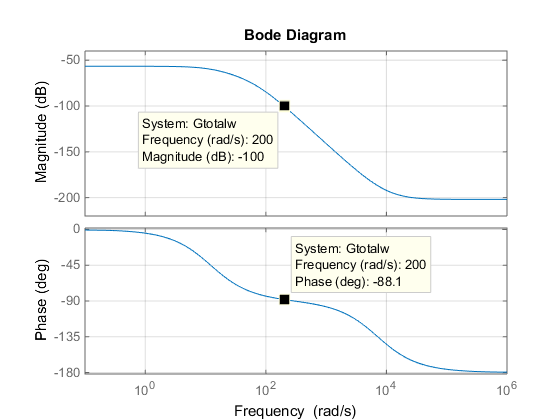
\includegraphics[scale=0.8]{diag_bode_planta_en_w.png}
	\caption{Diagrama de Bode de lazo abierto $G_c*GH_{T}(w)$ con $M=30\:kg$.}
	\label{fig:bode_digital}
\end{figure}

\begin{figure}[H]
	\centering
	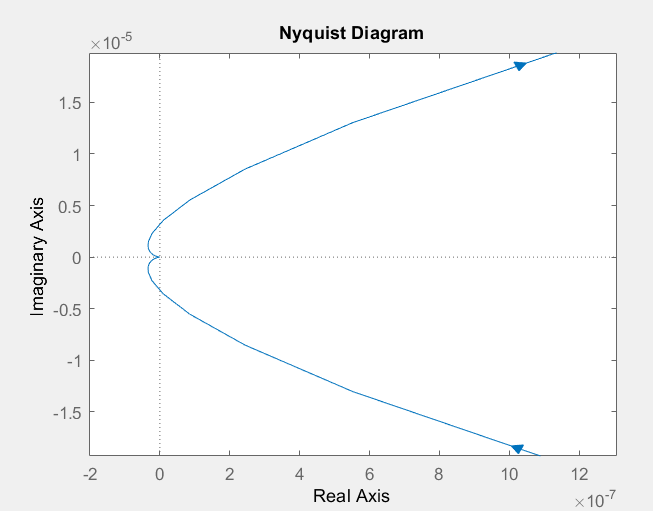
\includegraphics[scale=0.75]{Nyquist-lazo-abierto-digital.png}
	\caption{Diagrama de Nyquist de $G_c*GH_{T}(w)$ con $M=30\:kg$.}
	\label{fig:nyquist-lazo-abierto-digital}
\end{figure}

Como la transferencia de la planta $GH_T$ tiene un polo en el semiplano derecho del plano ``w'' no es posible determinar su estabilidad por medio del diagrama de Bode. Por lo tanto, se analiza la estabilidad por medio del criterio de Nyquist.

Como se observa en el diagrama en bloques de la figura \ref{fig:diag-interno_dig}, para compensar al sistema se planteó una realimentación negativa. Por lo tanto, para analizar su estabilidad según Nyquist se deben determinar la cantidad de giros (N) de $G_c*GH_T$ alrededor del punto $-1+j0$ en la figura \ref{fig:nyquist-lazo-abierto-digital} y la cantidad de polos (P) en el semiplano derecho de la función transferencia $G_c*GH_T$. El sistema resultará estable si se cumple la condición \ref{eq_condicion_Nyquist}, donde Z representa la cantidad de ceros en el semiplano derecho de $1+G_c*GH_T(w)$.

\begin{equation}\label{eq_condicion_Nyquist}
	Z=N+P=0
\end{equation}


Debido a que $GH_T$ tiene un polo en el semiplano derecho ($P=1$) y no hay giros alrededor del punto $-1+j0$ ($N=0$), resulta que $Z=1$. Por lo tanto, la transferencia de lazo cerrado ($TLC_{interna}$) presenta un comportamiento inestable. En la figura \ref{fig:nyquist-lazo-abierto-digital} se puede observar que no existe ningún valor de $K>0$ que haga que el contorno de $G_c*GH_T$ rodee el punto $-1+j0$. Por lo tanto, se propone implementar un compensador con $K<0$, para invertir el contorno de $G_c*GH_T$. Esto resulta equivalente a considerar $K>0$ y usar realimentación positiva en el lazo de control interno. De esta forma se obtiene el diagrama en bloques de la figura \ref{fig:diag-interno_dig_realimentacion_positiva}.


\begin{figure}[H]
	\centering
	\tikzset{%
	buffer/.style={
		draw,
		shape border rotate=270,
		regular polygon,
		regular polygon sides=3,
		fill=blue!20,
		node distance=2cm,
		minimum height=4em
	}
}

\tikzstyle{block} = [draw, fill=blue!20, rectangle, 
minimum height=2.5em, minimum width=3em]

%Acá se define eñ diagrama en bloques completo
\begin{tikzpicture}[auto, node distance=1.5cm,>=latex']
	% We start by placing the blocks
	\node [input, name=input] {};
	\node [sum, right of=input, node distance=1.5cm] (suma_interna) {+};
	\node[block, right=of suma_interna] (interno) {$G_c$};
	\node [block, right=of interno] (gil) {$G_{IL}$};
	\node [block, right=of gil] (planta) {$G_p$};
	\node [block, below=of gil] (realimentacion_interna) {$H_{estim}$};
	
	
%	\node [block, right of=suma] (amplificador) {$A(s)$};
	\node [output, right of=planta, node distance=3cm] (output) {};
%	\node [block, below of=amplificador] (realimentacion) {$H(s)$};
%	
%	
%	% Once the nodes are placed, connecting them is easy. 
%	\draw [draw,->] (input) -- node[pos=0.2]{$V_{y_{ref}}$} (F);
	\draw [draw,->] (input) -- node[pos=0.2]{$V_{ref_c}$} node[pos=0.9]{$+$}(suma_interna);

	\draw [draw,->] (suma_interna) -- node{$Ve_{int}$} (interno);
	\draw [draw,->] (interno) -- node{$V_{IL{ref}}$} (gil);
	\draw [draw,->] (gil) -- node{$I_L$} (planta);
	\draw [draw,->] (planta) -- node[name=y]{$Y_g$} (output);
%	\draw [draw,->] (amplificador) -- node[name=y]{$V_{deriv}$} (output);
	\draw [->] (y) |- (realimentacion_interna);
	\draw [->] (realimentacion_interna) -| node[pos=0.25]{$V_{estim}$}  node[pos=0.99]{$-$} (suma_interna);
%	\draw [->] (y) |- (realimentacion_externa);
%	\draw [->] (realimentacion_externa) -| node[pos=0.25]{$V_{estim}$} node[pos=0.99]{-} (suma_externa);
\end{tikzpicture}
	\caption{Diagrama en bloques del lazo de compensación interno.}	\label{fig:diag-interno_dig_realimentacion_positiva}
\end{figure}

\colorbox{red}{rehacer diagrama con relaimentacion positiva}

La realimentación positiva se genera al sumar la señal $Y_g$ con la señal de entrada del sistema. La transferencia de lazo cerrado del diagrama en bloques ahora se define como:

\begin{equation}
	TLC_{interna}=\frac{Y_g[m]}{V_{ref_c}[V]}=\frac{G_c*G_T}{1-G_c*G_T}
\end{equation}

Siguiendo el criterio de estabilidad de Nyquist, al utilizar realimentación positiva, la cantidad de giros (N) debe analizarse alrededor del punto $1+j0$. Si estos son en sentido horario, N será positivo, caso contrario será negativo. Al variar el valor de K, es posible hacer que el punto $1+j0$ quede contenido en la zona 1 o en la zona 2 de la figura \ref{fig:nyquist-con-zonas_digital}. 

\begin{figure}[H]
	\centering
	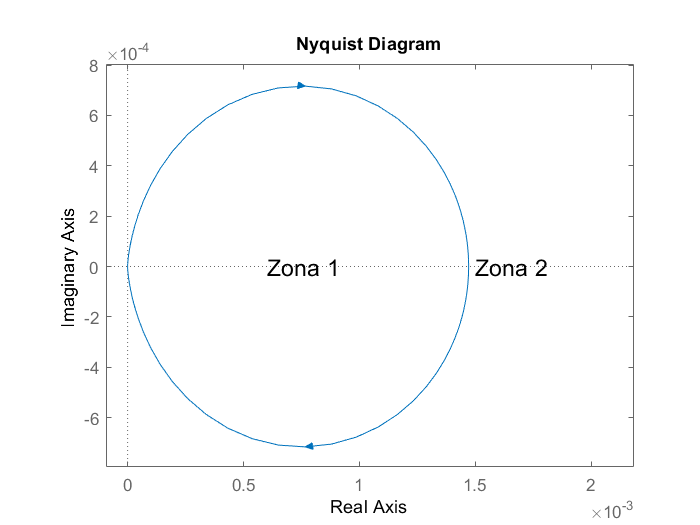
\includegraphics[scale=0.75]{Nyquist-lazo-abierto-digital-zonas.png}
	\caption{Diagrama de Nyquist con zonas marcadas.}
	\label{fig:nyquist-con-zonas_digital}
\end{figure}

Si el punto queda dentro de la zona 1, el número de giros es $N=1$. Por lo tanto, se plantea:

\begin{equation*}
	Z = N + P = 2
\end{equation*}


Si el punto queda dentro de la zona 2, el número de giros es $N=0$. Por lo tanto, se plantea:

\begin{equation*}
	Z = N + P = 1
\end{equation*}

Debido a que en ambas zonas Z resulta mayor que cero, el sistema realimentado no puede ser estabilizado con ningún valor de K. Para lograrlo se debe implementar un compensador $G_c$ que sea capaz de generar una zona en el diagrama de Nyquist donde exista un giro alrededor de $1 + j0$ en sentido antihorario de forma tal que $N=-1$ y resulte $Z=0$. Para ello, es necesario aumentar la fase para que pueda superar el valor de 0$\mathrm{{}^\circ}$. Para que esto se cumpla, el diagrama de Nyquist debe tener una forma como la  mostrada en la figura \ref{fig:nyquist-deseado-dig}.

\begin{figure}[H]
	\centering
	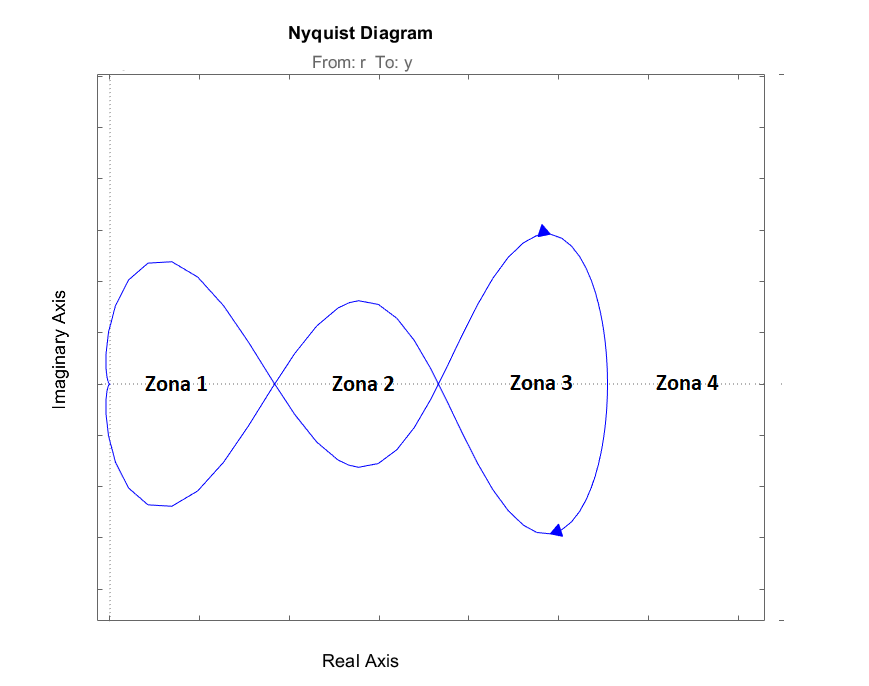
\includegraphics[scale=0.7]{Nyquist-deseado-dig.png}
	\caption{Diagrama de Nyquist deseado.}
	\label{fig:nyquist-deseado-dig}
\end{figure}

De esta manera se identifican cuatro zonas en las que puede estar ubicado el punto $1+j0$. Sin embargo, solo en la zona 2 se genera un giro en sentido antihorario ($N=-1$) como es deseado, por lo que resulta:

\begin{equation*}
	Z = N + P = 0
\end{equation*}

%Para lograr el comportamiento del sistema como en la figura 	\ref{fig:nyquist-deseado-analog} se debe tener en cuenta que el m\'{o}dulo de la transferencia de lazo abierto en el primer cruce de la fase por 0$\mathrm{{}^\circ}$ debe ser mayor a $0\:dB$ y, en el segundo cruce, menor. Para ello, se propone implementar un compensador por adelanto de fase.

A continuación se diseñará el compensador $G_c$ para lograr que el diagrama de Nyquist tenga la forma deseada y así, estabilizar el sistema.

\subsubsection{Diseño del compensador}

Para lograr el comportamiento del sistema como en la figura 	\ref{fig:nyquist-deseado-dig} se utilizará una estrategia de compensación por adelanto de fase. Esta consiste en observar el diagrama de bode de la figura \ref{fig:bode_digital} y elegir una frecuencia en la que se desee aumentar la fase para lograr la estabilidad. Se debe tener en cuenta que el módulo de la transferencia de lazo abierto en el primer cruce de la fase por 0$\mathrm{{}^\circ}$ debe ser mayor a $0\:dB$ y, en el segundo cruce, menor. 

De esta forma, al observar la figura \ref{fig:bode_digital} se decide generar un adelanto de fase de por lo menos 100° en la frecuencia $200\:r/s$. Esto se logra mediante el uso de un compensador compuesto por dos redes de adelanto de fase de 65$\mathrm{{}^\circ}$ cada una. 

Una red de adelanto de fase está compuesta por un polo ($W_p$) y un cero ($W_c$), de manera que el cero se encuentra a una frecuencia menor que el polo, permitiendo un aumento de fase a la frecuencia deseada $W_0$. Su transferencia es la siguiente:

\begin{equation} \label{eq_tf_adelanto_dig}
	G_{af}(w)=\alpha*\frac{(w + W_c)}{(w + W_p)}
\end{equation}

\noindent De esta forma, las ecuaciones de diseño resultan:

\begin{equation*}
	\begin{aligned}
		&W_0 =200\:r/s\\
		&{\varphi }_{max} =65\textrm{°}\\
		&\alpha =\frac{1+sen({\varphi }_{max})}{1-sen{(\varphi }_{max})}=20.346\\
		&W_c =\frac{W_0}{\sqrt{\alpha }}=\ 44.3\:r/s\\
		&W_p =\sqrt{\alpha }*W_0=902.1\: r/s\\
	\end{aligned}
\end{equation*} 
\noindent Finalmente, agregando una ganancia K y considerando las dos redes de adelanto de fase, se llega a la transferencia del controlador:

\begin{equation}  
	G_c(s)=K*{[20.346*\frac{(s+44.3)}{(s+902.1)}]}^2
	\label{eq:transferencia-del-compensador}
\end{equation} 

En la figura \ref{fig:bode-compensado-para-k-1} se muestra el diagrama de bode de ${GH}_T(w)*G_c(w)$ con $K=1$. Se puede observar que la ganancia $K$ puede adoptar valores desde $64\:dB$ hasta $88.6\:dB$. Al considerar que el sistema debe soportar una masa variable entre $1\:kg$ y $30\:kg$, y que la ganancia de la transferencia de la planta para $1\:kg$ es de $5.5$ veces ($14\:dB$) mayor que para $30\:kg$, se debe adoptar una ganancia del compensador que mantenga la estabilidad para estos dos casos. Es decir, la ganancia m\'{i}nima es de $64\:dB$ y la m\'{a}xima es de $88.6\:dB - 14\:dB = 74.6\:dB$. Por lo tanto, se elige que el cruce por cero de la ganancia se encuentre ahora en $88\:rad/s$, lo que significa que $K=68.4\:dB\ \equiv \ 2630\:veces$.

\begin{figure}[H]
	\centering
	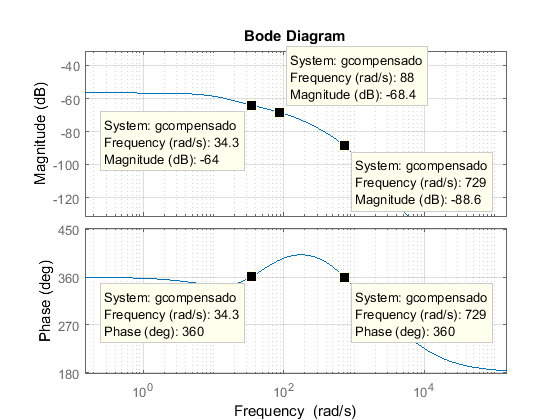
\includegraphics[scale=0.85]{Bode-compensado-para-k-1.png}
	\caption{Diagrama de Bode de $GH_T(w)*G_c(w)$ para $K=1$ y $M=30\:kg$.}
	\label{fig:bode-compensado-para-k-1}
\end{figure}
 
En la figura \ref{fig:bode-compensado-para-k-2630} se muestra el diagrama de Bode al considerar la ganancia del compensador. En ella se puede observar que se  cumple con el criterio de estabilidad, puesto que en el primer cruce por 0°, la magnitud es mayor a $0\:dB$ y en el segundo cruce, menor. Además, en la figura \ref{fig:nyquist-para-k-2630} se grafica el diagrama de Nyquist para el sistema con el compensador. En él se puede ver que el punto $1+j0$ queda dentro de la zona en la que $N=-1$, que resulta en $Z=0$.

\begin{figure}[H]
	\centering
	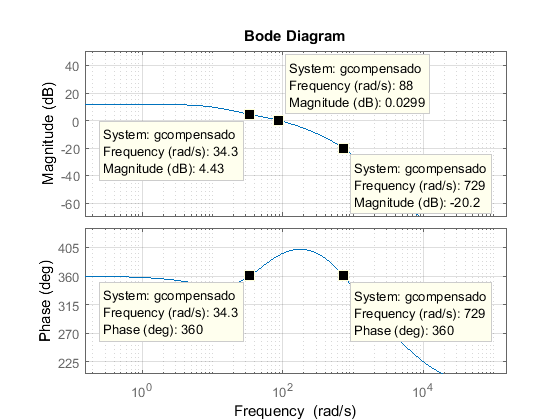
\includegraphics[scale=0.75]{Bode-compensado-para-k-2630.png}
	\caption{Diagrama de Bode de $GH_T(w)*G_c(w)$ para $K=2630$ y $M=30\:kg$.}
	\label{fig:bode-compensado-para-k-2630}
\end{figure}

\begin{figure}[H]
	\centering
	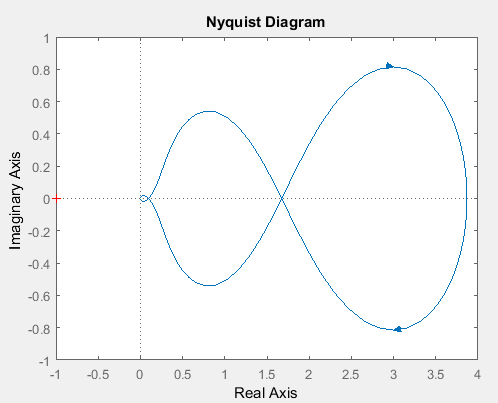
\includegraphics[scale=0.55]{Nyquist-para-k-2630.png}
	\caption{Diagrama de Nyquist de $GH_T(w)*G_c(w)$ para $K=2630$ y $M=30\:kg$.}
	\label{fig:nyquist-para-k-2630}
\end{figure}

\subsubsection{Análisis de estabilidad con masa mínima}


Se verifica la estabilidad del sistema  para el caso en que la masa sea de $1\:kg$ con el compensador previamente diseñado. Para ello, se analizan los diagramas de Bode y Nyquist mostrados en las figuras \ref{fig:bode-para-M-1Kg} y \ref{fig:nyquist-para-M-1Kg}. A partir de ellos, es posible verificar que el sistema resulta estable para todo el rango de masas en el que opera el sistema. Sin embargo, se puede observar que el margen de fase es menor que 45°, por lo que el sistema puede presentar un transitorio con oscilaciones amortiguadas. A raíz de esto, se propone implementar un lazo de control externo que permita mejorar dicha respuesta.


\begin{figure}[H]
	\centering
	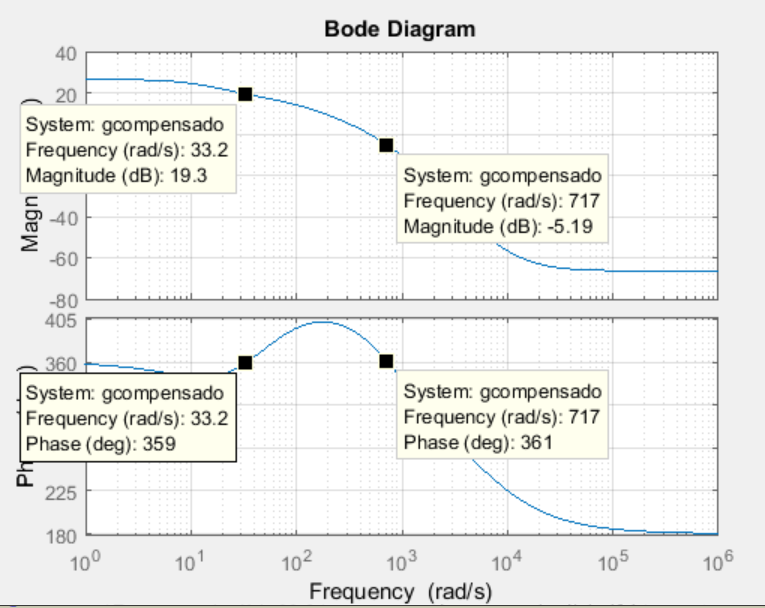
\includegraphics[scale=0.85]{Bode-para-M-1Kg.png}
	\caption{Diagrama de Bode de $GH_T(w)*G_c(w)$ para $M=1\:kg$.}
	\label{fig:bode-para-M-1Kg}
\end{figure}

\begin{figure}[H]
	\centering
	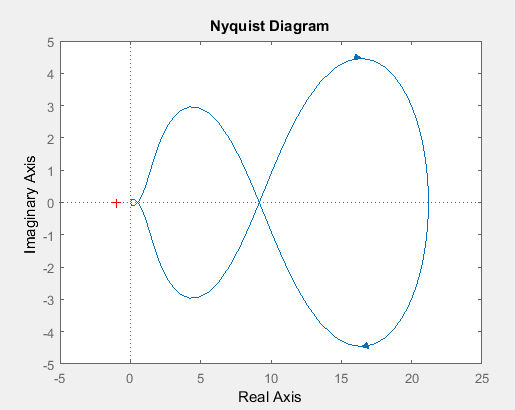
\includegraphics[scale=0.6]{Nyquist-para-M-1Kg.png}
	\caption{Diagrama de Nyquist de $GH_T(w)*G_c(w)$ para $M=1\:kg$.}
	\label{fig:nyquist-para-M-1Kg}
\end{figure}

\subsubsection{Transferencia de lazo cerrado}

Finalmente se puede expresar la función transferencia del lazo de control interno como:
%
%-3.6301e05 (s+1000) (s+44.3)^2
%------------------------------------------------------------------
%(s+304.3) (s+115.6) (s^2 + 44.84s + 2588) (s^2 + 2352s + 1.498e06)


\begin{equation}
	TLC_{interna}(w)=\frac{Y_g}{V_{ref_c}}=\frac{G_c*G_T}{1-G_c*G_T}
	%	\frac{-3.6301*}{den}
\end{equation}

Para el caso de trabajar con masa de $30\:kg$, la $TLC_{interna}$ resulta:
%
%  -8.7319e-05 (s+1.237e04) (s-1.238e04) (s-7143) (s+44.34)^2
%----------------------------------------------------------
%(s+1197) (s+471.1) (s+103.6) (s^2 + 44.34s + 2383)

\begin{equation*}
	\resizebox{.99\hsize}{!}
	{
		$
		TLC_{interna}(w)=\frac{-8.73*10^{-5} (w+1.24*10^4) (w-1.24*10^4) (w-7143) (w+44.34)^2}{(w+1197) (w+471.1) (w+103.6) (w^2 + 44.34w + 2383)}
		$
	}
\end{equation*}


Para el caso de trabajar con masa de $1\:kg$, resulta:

% -0.00047808 (s+1.237e04) (s-1.238e04) (s-7143) (s+44.34)^2
%----------------------------------------------------------
%(s+1527) (s^2 + 88.75s + 2128) (s^2 + 196.9s + 3.014e05)

\begin{equation*}
	\resizebox{.99\hsize}{!}
	{
		$
		TLC_{interna}(w)=\frac{-4.78*10^{-4} (w+1.24*10^4) (w-1.24*10^4) (w-7143) (w+44.34)^2}{(w+1527) (w^2 + 88.75w + 2128) (w^2 + 196.9w + 3.01*10^5)}	
		$
	}
\end{equation*}



En las figuras \ref{fig:ubicacion_polos_y_ceros_dig} y \ref{fig:ubicacion_polos_y_ceros_1kg_dig} se muestra la ubicación de los polos y ceros de la $TLC_{interna}$ para el caso de masa de $30\:kg$ y $1\:kg$, respectivamente. En ellas se ve que todos los polos se encuentran en el semiplano izquierdo. 

\begin{figure}[H]
	\centering
	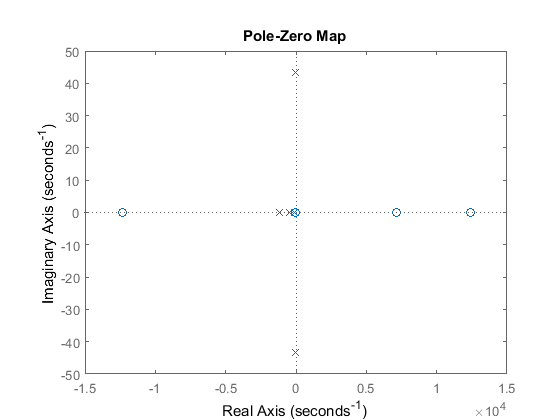
\includegraphics[scale=0.85]{ubicacion_polos_ceros_dig.png}
	\caption{Ubicación de polos y ceros de la transferencia de lazo cerrado interna con $M=30\:kg$.}
	\label{fig:ubicacion_polos_y_ceros_dig}
\end{figure}

\begin{figure}[H]
	\centering
	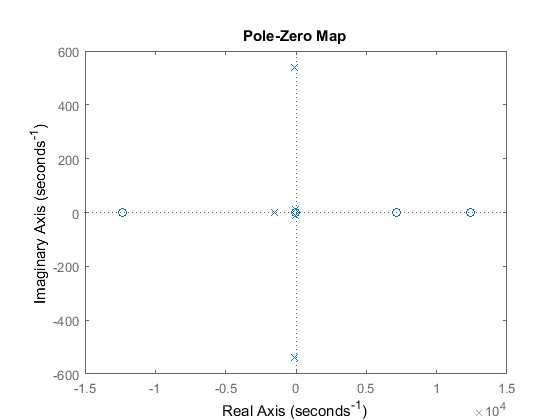
\includegraphics[scale=0.85]{ubicacion_polos_ceros_1kg_dig.png}
	\caption{Ubicación de polos y ceros de la transferencia de lazo cerrado interna con $M=1\:kg$.}
	\label{fig:ubicacion_polos_y_ceros_1kg_dig}
\end{figure}

Es importante notar que la ganancia de la transferencia de lazo cerrado en ambos casos es negativa. Esto debe tenerse en cuenta para el diseño del lazo de compensación externo.


\subsubsection{Cálculo de los coeficientes del controlador}

Para implementar el algoritmo de control en el microcontrolador se aplica la transformada bilineal inversa a la transferencia del compensador por adelanto de fase $G_c(w)$. Por lo tanto, se obtiene:

% 8.69e05 z^2 - 1.716e06 z + 8.477e05
%-----------------------------------
%z^2 - 1.551 z + 0.6018
%
%
%  8.69e05 - 1.716e06 z^-1 + 8.477e05 z^-2
%---------------------------------------
%1 - 1.551 z^-1 + 0.6018 z^-2

\begin{equation} \label{eq_coeficientes_interno} 
	G_c(z)=\ \ \frac{U(z)}{e(z)}=\frac{8.69*10^5- 1.72*10^6z^{-1} + 8.48*10^5z^{-2}}{1-1.551 z^{-1} + 0.6018 z^{-2}}\  
\end{equation} 



\colorbox{red}{Ver si es necesario poner aca la ecuacion en diferencias}



\colorbox{red}{Aca empieza lazo externo}
 Se plantea un lazo de realimentaci\'{o}n externo como se muestra en la  figura \ref{fig:diagrama-del-sistema-completo}.

\begin{figure}[H]
	\centering
	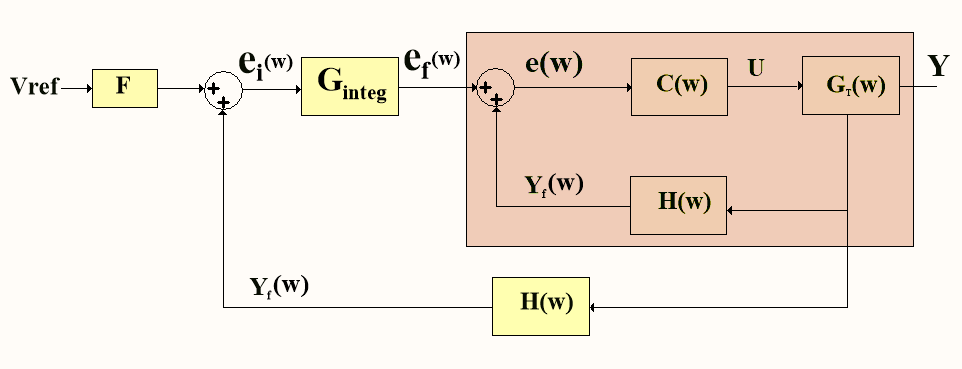
\includegraphics[scale=0.4]{Diagrama-del-sistema-completo.png}
	\caption{Diagrama del sistema completo.}
	\label{fig:diagrama-del-sistema-completo}
\end{figure}


 En el lazo de realimentaci\'{o}n interno act\'{u}a el compensador por adelanto de fase dise\~{n}ado previamente y, en el externo, un controlador del tipo integral. De esta forma, se logra suavizar la respuesta al escal\'{o}n del sistema y eliminar el error en r\'{e}gimen permanente.


 Para el an\'{a}lisis se considera $H(w)=1$ como realimentaci\'{o}n. La cadena de avance con masa de $30\:kg$ es:

\[G(W)[M=30]=Tlc(W)[M=30]*G_{integ}\] 

 Se  plantea un compensador del tipo :

\[G_{integ}\ =\ k_{int}\ *\ \frac{1}{w}\] 

 La ganancia del bloque de entrada (F) se establece igual a la ganancia del estimador (H) pero cambiada de signo, debido a que la transferencia de lazo cerrado tiene una inversi\'{o}n de fase. Por lo tanto, se toma $F=-H=-1$.

 Inicialmente se adopta $k_{int} = 1$ para poder evaluar, por medio de lugar de ra\'{i}ces mostrado en la figura \ref{fig:lugar-de-raices-con-integrador}, la estabilidad del sistema. Para este lazo de realimentaci\'{o}n externo tambi\'{e}n debe utilizarse realimentaci\'{o}n positiva puesto que los polos de la TLC interna est\'{a}n en el semiplano izquierdo pero presenta una inversi\'{o}n de signo.


\begin{figure}[H]
	\centering
	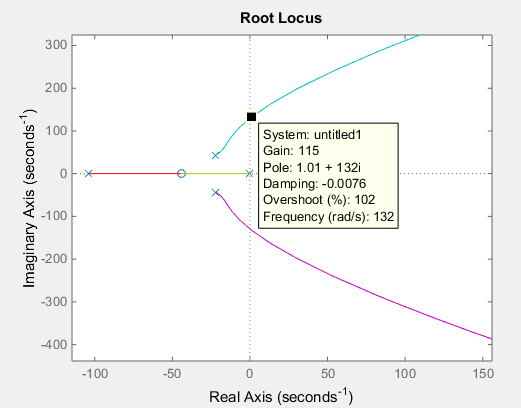
\includegraphics[scale=0.6]{Lugar-de-raices-con-integrador.png}
	\caption{Lugar de raíces con el integrador.}
	\label{fig:lugar-de-raices-con-integrador}
\end{figure}


 En la figura \ref{fig:lugar-de-raices-con-integrador} se puede observar que, para que se mantenga la estabilidad del sistema, la ganancia del integrador ($K_{int}$) debe ser menor a 115. Por lo tanto, en la figura \ref{fig:respuesta-al-escalon-con-k-1-M-30} se muestra la respuesta al escal\'{o}n del sistema compensado con el integrador para una ganancia de $K_{int}=1$.  Es posible observar que, si bien no presenta oscilaciones, el tiempo de establecimiento es de aproximadamente $3\:s$. Por lo tanto, se decide aumentar el valor de ganancia hasta obtener una relaci\'{o}n aceptable entre el tiempo de respuesta y el sobrepico.


\begin{figure}[H]
	\centering
	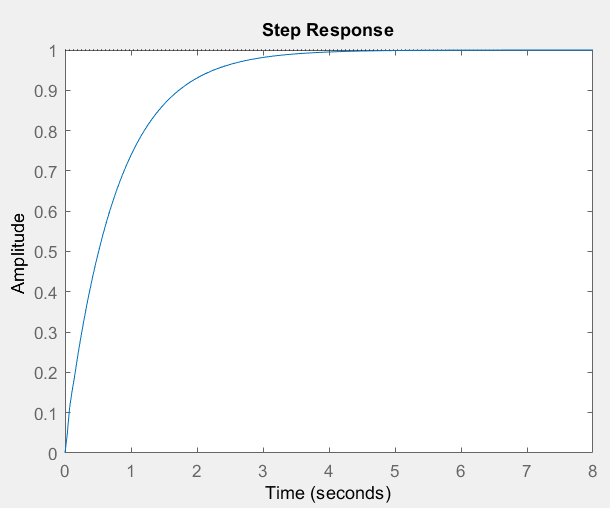
\includegraphics[scale=0.85]{Respuesta-al-escalon-con-k-1-M-30.png}
	\caption{Respuesta al escalón con integrador con $K_{int} =1$ y $M=30\:kg$.}
	\label{fig:respuesta-al-escalon-con-k-1-M-30}
\end{figure}


 En la figura \ref{fig:respuesta-al-escalon-con-k-20-M-30}, se observa la respuesta al escal\'{o}n para una ganancia del integrador de $K_{int}=20$ que resulta en un tiempo de establecimiento de $0.22\:s$ y un \textsl{overshoot} de 4.41\%. Por lo tanto, se adopta este valor de ganancia para el dise\~{n}o del integrador.

\begin{figure}[H]
	\centering
	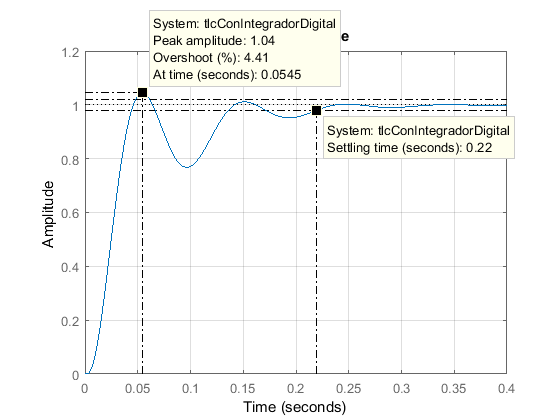
\includegraphics[scale=0.85]{Respuesta-al-escalon-con-k-20-M-30.png}
	\caption{Respuesta al escalón con integrador para $K_{int} =20$ y $M = 30\:kg$.}
	\label{fig:respuesta-al-escalon-con-k-20-M-30}
\end{figure}


 La respuesta al escal\'{o}n cuando la masa es de $1\:kg$ se muestra en la figura \ref{fig:respuesta-al-escalon-con-k-20-M-1}. All\'{i} se puede observar que el tiempo de crecimiento es de $0.104\:s$ y el de establecimiento de $0.196\:s$. Adem\'{a}s, es posible notar que no presenta sobrepicos.



\begin{figure}[H]
	\centering
	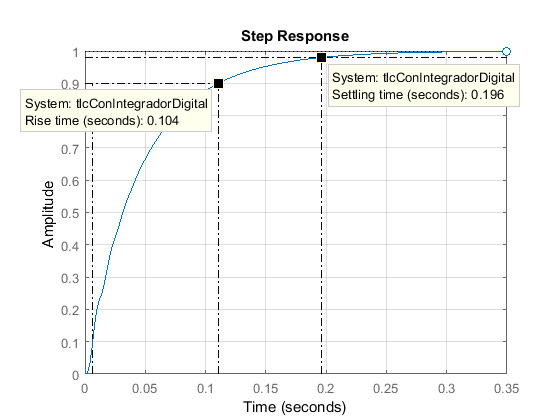
\includegraphics[scale=0.85]{Respuesta-al-escalon-con-k-20-M-1.png}
	\caption{Respuesta al escalón con integrador para $K_{int} =20$ y $M=1\:kg$.}
	\label{fig:respuesta-al-escalon-con-k-20-M-1}
\end{figure}


\section{Cálculo de los coeficientes del controlador}

 Para implementar el algoritmo de control en el microcontrolador se aplica la transformada bilineal inversa a las transferencias del compensador por adelanto de fase $C(w)$ y al integrador $G_{integ}(w)$.

 Por lo tanto, se obtiene:

\begin{equation} \label{GrindEQ__5_6_} 
	C(z)=\ \ \frac{U(z)}{e(z)}=\frac{8.6896*10^5(z-0.9877)^2}{\ (z-0.7757)^2}\  
\end{equation} 

\begin{equation} \label{GrindEQ__5_7_} 
	G_{integ}(z)=\frac{e_f(z)}{e_i(z)}\ =\frac{0.0028(\ z\ +\ 1)}{\ (z\ -\ 1)} 
\end{equation} 

 Si se considera $H(z)=1$ se obtiene que:

\begin{equation} \label{GrindEQ__5_39_} 
	e(z)=e_f(Z)+Y_f(z) 
\end{equation} 

\begin{equation} \label{GrindEQ__5_40_} 
	e_i(z)=F*Vref+Y_f(z) 
\end{equation} 


 Al aplicar la partir de las ecuaciones \ref{GrindEQ__5_6_} y \ref{GrindEQ__5_7_} se obtiene las expresiones a implementar en el microcontrolador:

\begin{equation} 
	\begin{aligned}\label{eq_U-coef}
	U[n]=&8.651*10^5e[n]-\ 1.709*10^6e[n-1]+\ 0.843*10^6e[n-2]+\\
		 &+1.5514\ U[n-1]-\ 0.60171U[n-2]\\ 
	\end{aligned}
\end{equation}

\begin{equation} \label{eq_e-coef} 
	e_f[n]=0.0028*e_i[n]\ +\ {0.0028*e}_i[n-1]+e_f[n-1] 
\end{equation} 


 Luego, para dejar el algoritmo de control en funci\'{o}n de las entradas del sistema, se debe reemplazar en las ecuaciones \ref{eq_U-coef} y \ref{eq_e-coef} las expresiones mencionadas en las ecuaciones \ref{GrindEQ__5_10_} y \ref{GrindEQ__5_11_}

\begin{equation} \label{GrindEQ__5_10_} 
	e[n]=e_f[n]+Y_f[n] 
\end{equation} 

\begin{equation} \label{GrindEQ__5_11_} 
	e_i[n]=F*Vref+Y_f[n] 
\end{equation} 

\section{Conexi\'{o}n entre el PCB y el microcontrolador}

 Se utiliza un conector tipo DB9 hembra como v\'{i}a de conexi\'{o}n para las distintas salidas y entradas digitales. Adem\'{a}s, en la placa se dispone de un led que se enciende cuando  se detecta una correcta conexi\'{o}n con el microcontrolador.







